\documentclass{article}

% NeurIPS 2026 format, double-blind workshop mode (anonymous + line numbers + workshop footer).
% For the camera-ready, swap [dblblindworkshop] -> [final] and de-anonymize the author block.
\usepackage[dblblindworkshop, nonatbib]{neurips_2026}
\usepackage[numbers]{natbib}
\workshoptitle{Grounded and Faithful Vision-Language Models for Real-World Deployment (VLM4RWD)}

\usepackage[export]{adjustbox}
\usepackage[ruled]{algorithm2e}
\usepackage[inline, shortlabels]{enumitem}
\usepackage[T1]{fontenc}
\usepackage{hyperref}
\usepackage{microtype}
\usepackage{pifont}
\usepackage{xcolor}
\usepackage{xurl}
% Figures and Tables
\usepackage{graphicx}
\usepackage{booktabs}
\usepackage{tabularray}
% Monospaced Code Blocks
\usepackage{listings}
% Math Packages
\usepackage{amsmath, amsfonts}
\usepackage{nicefrac}

\UseTblrLibrary{booktabs}

\lstset{
  backgroundcolor=\color{white},   % choose the background color; you must add \usepackage{color} or \usepackage{xcolor}; should come as last argument
  basicstyle=\ttfamily,            % the size of the fonts that are used for the code
  breakatwhitespace=false,         % sets if automatic breaks should only happen at whitespace
  breaklines=true,                 % sets automatic line breaking
  captionpos=b,                    % sets the caption-position to bottom
  columns=fullflexible,            % reduce the column spacing
  commentstyle=\color{gray},       % comment style
  deletekeywords={},               % if you want to delete keywords from the given language
  escapeinside={\%*}{*)},          % if you want to add LaTeX within your code
  extendedchars=true,              % lets you use non-ASCII characters; for 8-bits encodings only, does not work with UTF-8
  frame=none,                      % adds no frame around the code
  keepspaces=true,                 % keeps spaces in text, useful for keeping indentation of code (possibly needs columns=flexible)
  keywordstyle=\color{blue},       % keyword style
  language=C++,                    % the language of the code
  morekeywords={},                 % if you want to add more keywords to the set
  numbers=none,                    % where to put the line-numbers; possible values are (none, left, right)
  numbersep=5pt,                   % how far the line-numbers are from the code
  numberstyle=\color{black},       % the style that is used for the line-numbers
  rulecolor=\color{black},         % if not set, the frame-color may be changed on line-breaks within not-black text (e.g. comments (green here))
  showspaces=false,                % show spaces everywhere adding particular underscores; it overrides 'showstringspaces'
  showstringspaces=false,          % underline spaces within strings only
  showtabs=false,                  % show tabs within strings adding particular underscores
  stepnumber=1,                    % the step between two line-numbers. If it's 1, each line will be numbered
  stringstyle=\color{red},         % string literal style
  tabsize=4,                       % sets default tabsize to 4 spaces
}

\makeatletter
\newcommand{\ssymbol}[1]{\@fnsymbol{#1}}
\newcommand{\romanNumeral}[1]{\expandafter\@slowromancap\romannumeral #1@}
\makeatother

\usepackage{mathtools}
\usepackage{siunitx}
\sisetup{detect-weight=true, detect-family=true}

\newcommand{\ci}[2]{{\footnotesize[#1,\,#2]}}   % 95\% CI helper

\title{Same Eye, Different Scanner: A Decision-Reliability Benchmark for\\
Frontier VLMs and OCT Foundation Models in Glaucoma}

\author{%
  Anonymous Author(s)\\
  Affiliation\\
  \texttt{anonymous@example.com}%
}

\begin{document}

\maketitle

% ======================================================================================
%  Scanner-shift OCT benchmark / VLM4RWD — body (rebuilt from reports/oct_format_paper_outline.md)
% ======================================================================================

\begin{abstract}
A glaucoma-OCT reader used across providers should give the same eye the same diagnosis whatever scanner
acquired the image. In practice, however, OCT measurements are not interchangeable across scanners, so a
model's decision can change even though the eye is unchanged. We ask whether prompted frontier vision-language models (VLMs) and specialist OCT foundation models (FMs)
keep a faithful, calibrated decision when the scanner changes. We build a benchmark that applies the scanner change
as a same-eye image transform calibrated to measured cross-scanner disagreement. Because each eye is scored before
and after, the scanner effect is de-confounded from patient differences while the images and labels stay real. We
score the decision at a fixed operating point (a single decision threshold) by its decision-flip rate, change in
sensitivity, and expected calibration error (ECE), with bootstrap confidence intervals (CIs) on the decision metrics. Four results follow.
(1)~Prompted frontier VLMs are the weakest and most overconfident above-chance readers on the raw B-scan (AUC
\num{0.61}--\num{0.69}). Their ECE is roughly 5--10$\times$ the best FM's for the Gemini and GPT families (Claude
Opus~5 a better-calibrated exception); smaller open-weights and medical-specialist VLMs are near chance
(\num{0.41}--\num{0.59}).
(2)~Rendered as a color thickness map, the stronger VLMs reach the level of the strong generic-FM and CNN readers
(AUC \num{0.83}--\num{0.84}), far above their raw-B-scan scores. The small open models do not recover, so what lets a
VLM read the scan is the display format together with a capable base, not model size alone (a cross-dataset
comparison). (3)~A scanner change can break the decision while discrimination is intact:
$\Delta$AUC$\approx$0 while the diagnostic decision flips and specificity can collapse, invisible to AUC-only
evaluation. (4)~Reliability tracks the input representation and pretraining breadth, not model size: across a
26M--197M CNN sweep the largest model is steadiest on neither axis, and on the thickness-map axis a 98k-parameter
from-scratch CNN matches 300M-parameter models on decision stability.
\end{abstract}

% ======================================================================================
\section{Introduction}
\label{sec:intro}

Glaucoma is a leading cause of irreversible blindness, projected to affect 111.8 million people by 2040
\citep{tham2014global} and often undiagnosed \citep{soh2021undetected}. Optical coherence tomography (OCT) of the
retinal nerve fiber layer (RNFL) is a standard
structural test, recommended for diagnosis by clinical practice guidelines \citep{gedde2021ppp}, and deep-learning
readers now detect glaucoma from OCT at the level of specialists \citep{ran2019oct}, increasingly via foundation
models \citep{zhou2023retfound}, producing one decision per eye: glaucoma or not. Prompted frontier vision-language models (VLMs) are being proposed as
general-purpose medical readers \citep{chen2024gmaimmbench, qin2024lmod}, attractive because they do not need task-specific training, but whether they are reliable enough for real deployment is largely untested.

That reliability is tested first by the scanner. Single-site care sidesteps the problem by repetition: the patient is
monitored on one machine and simply re-scanned when referred elsewhere. To meet rising demand
and prevent the follow-up delays that cause avoidable sight loss, clinical guidance is shifting glaucoma care to
virtual, cross-provider triage in which a single digital OCT, acquired in community optometry \citep{jindal2019}, is
shared and read remotely, with AI-assisted coordination \citep{girft2026glaucoma}. Automated readers that support the
decision are increasingly proposed to scale such screening and monitoring across providers
\citep{ting2019ai}, including teleophthalmology \citep{thomas2014teleglaucoma} and multi-site follow-up
\citep{niceng81, gedde2021ppp}. OCT, however, is scanner-dependent: the same eye yields different RNFL measurements
across scanners because segmentation and normative databases differ \citep{buchser2012}, and its raw B-scan
appearance varies with frame-averaging, speckle, and contrast \citep{schmitt1999speckle}. A reader deployed across
providers must therefore treat the scanner as a nuisance variable that does not move the decision: one whose
diagnosis tracks the scanner rather than the eye cannot support multi-provider care, whatever its single-scanner
accuracy.

Single-scanner accuracy cannot see this, and existing work covers only parts of the problem.
Cross-scanner claims for OCT foundation models are made on real cohorts where the scanner coincides with the patient group and are scored by
accuracy or AUC alone \citep{zhou2023retfound, liu2024octcubem, morano2025mirage}. Verbalized-overconfidence studies
use natural images and no clinical decision \citep{groot2024overconfidence}, and medical-VLM trustworthiness
benchmarks span modalities but omit any glaucoma decision under a scanner shift \citep{xia2024cares}. The closest glaucoma
study fine-tunes VLM encoders on a single scanner, with no shift, no decision metric, and no calibration
\citep{jalili2025tvst}. No prior benchmark combines a calibrated same-eye scanner shift, decision-level and
calibration metrics, and a VLM-versus-FM common ground.

We therefore introduce a benchmark that measures this cross-scanner decision reliability directly. We apply the scanner change
as a same-eye image transform calibrated to measured cross-scanner disagreement: published Bland--Altman limits of
agreement for thickness maps \citep{warner2011loa, blandaltman1986} and real per-vendor speckle for B-scans
\citep{schmitt1999speckle, bogunovic2019retouch}. Because the same eye is scored before and after, the scanner effect
is de-confounded from patient differences, and the images and labels stay real. We score
every reader at a fixed operating point by decision-flip, change in sensitivity, and calibration error, with
bootstrap confidence intervals (CIs) on the decision metrics. On this common ground we place prompted frontier VLMs, smaller open-weights and
medical-specialist VLMs, OCT and generic foundation models (FMs), a controlled ImageNet CNN model-size sweep, and a
from-scratch CNN.

\paragraph{Contributions.}
\begin{itemize}[leftmargin=1.2em, itemsep=1pt, topsep=1pt]
\item \textbf{A de-confounded benchmark and decision-level metric suite for scanner-change reliability}
  (\S\ref{sec:benchmark}). To our knowledge the first evaluation that asks whether a glaucoma-OCT reader keeps its
  decision across scanners with the scanner effect isolated from patient differences, scored by a calibration-aware
  metric suite (decision-flip, $\Delta$sens@spec, spec@shift, ECE; bootstrap CIs on the decision metrics) that
  single-scanner accuracy cannot provide, applied uniformly across the VLM, foundation-model, and CNN readers.
\item \textbf{Prompted frontier VLMs are the weakest and most overconfident above-chance readers of raw OCT} (\S\ref{sec:findings},
  F1). On the raw B-scan they fall below the specialist FMs and are badly miscalibrated (with Claude Opus~5 a
  better-calibrated exception), and smaller open-weights and medical-specialist VLMs are near chance, an unsafe
  default for clinical OCT reading.
\item \textbf{Frontier VLMs read a thickness map far better than a raw B-scan} (F2). The stronger frontier VLMs reach
  the strong generic-FM/CNN readers' level on the thickness-map task but fail on the B-scan task, pointing to input
  representation over model size or vendor; the gap is specific to general-purpose VLMs (a cross-dataset comparison we
  caveat in \S\ref{sec:discussion}).
\item \textbf{A scanner change can break the decision while discrimination holds} (F3). Discrimination can be
  unchanged ($\Delta$AUC$\approx$0) while the decision flips and specificity can collapse, a failure AUC-only
  evaluation cannot detect and only decision-level and calibration metrics reveal.
\item \textbf{Stability tracks representation and pretraining breadth, not model size} (F4). Across a one-family CNN
  model-size sweep, OCT and generic FMs, and a from-scratch network, tolerance to the scanner change is flat across
  model size: on the thickness-map axis a 98k-parameter CNN is CI-tied with the best CNNs and matches 300M-parameter models on
  decision stability.
\end{itemize}

% ======================================================================================
\section{Related work}
\label{sec:related}

Three lines of prior work are relevant to our question: the reliability of (medical) VLMs, cross-scanner
generalization of OCT models, and prompted VLMs for glaucoma.

\paragraph{Reliability and evaluation of (medical) VLMs.} Object-hallucination work showed that generative vision
models assert ungrounded content \citep{rohrbach2018chair, li2023pope}. Verbalized-probability elicitation, the
standard cross-model confidence denominator \citep{lin2022verbalized, tian2023calibration, xiong2024uncertainty}, is
weakly calibrated for frontier multimodal models: \citet{groot2024overconfidence} report GPT-4V and Gemini
overconfidence on natural images, in line with the broader result that predictive uncertainty degrades under
dataset shift \citep{ovadia2019shift}. On medical images, general-purpose and medical VLMs (e.g.\ LLaVA-Med
\citep{li2023llavamed}) remain well short of clinical-grade accuracy on broad medical benchmarks
\citep{chen2024gmaimmbench}, reason weakly about eye
images \citep{qin2024lmod}, and on glaucoma reach high accuracy
but poor sensitivity on fundus grading \citep{alryalat2024chatgpt}. Trustworthiness benchmarks such
as CARES score an over-confidence ratio across medical modalities \citep{xia2024cares}. None of these pair a clinical
decision with a calibrated scanner shift and a decision-level, calibration-aware metric, which is our focus.

\paragraph{OCT foundation models and cross-scanner generalization.} OCT-specific foundation models claim cross-scanner
transfer, but on real held-out cohorts where scanner coincides with cohort (a confound) and scored by accuracy or
AUC \citep{zhou2023retfound, liu2024octcubem, morano2025mirage}. A prior mitigation, cross-domain image translation,
can recover device-specific glaucoma-OCT accuracy \citep{belghith2025crossdomain}, but is validated by accuracy on
real cohorts, not by decision stability under a same-eye shift. More broadly, distribution shift, both naturally
occurring \citep{koh2021wilds} and synthetic \citep{hendrycks2019corruptions}, is a mature benchmark topic, and
retinal AI has been externally validated across fundus cameras \citep{tsai2022crosscamera}, the same varying-hardware
design we adopt. We differ by applying the scanner as a calibrated same-eye transform, which de-confounds it from
cohort by construction, and by scoring the decision and its calibration rather than accuracy alone.

\paragraph{Prompted VLMs for glaucoma (the closest neighbor).} \citet{jalili2025tvst} fine-tune VLM vision encoders
on a single scanner and find them competitive with OCT FMs (LLaVA \num{0.92} vs.\ RETFound \num{0.91}), with no
distribution shift, decision metric, or calibration. The same group's GPT-4V study \citep{jalili2024gpt4v} is the
closest prompted-frontier-VLM precedent, but it grades fundus images and reports accuracy only, with no scanner
shift or calibration. Our claim is instead about
\emph{prompted} frontier VLMs (zero- or few-shot, verbalized probability) under a calibrated scanner shift: a
fine-tuned encoder can match a specialist while a prompted generalist stays weak and overconfident, so the two
settings measure different deployment modes.

% ======================================================================================
\section{The benchmark}
\label{sec:benchmark}

\begin{figure}[t]
  \centering
  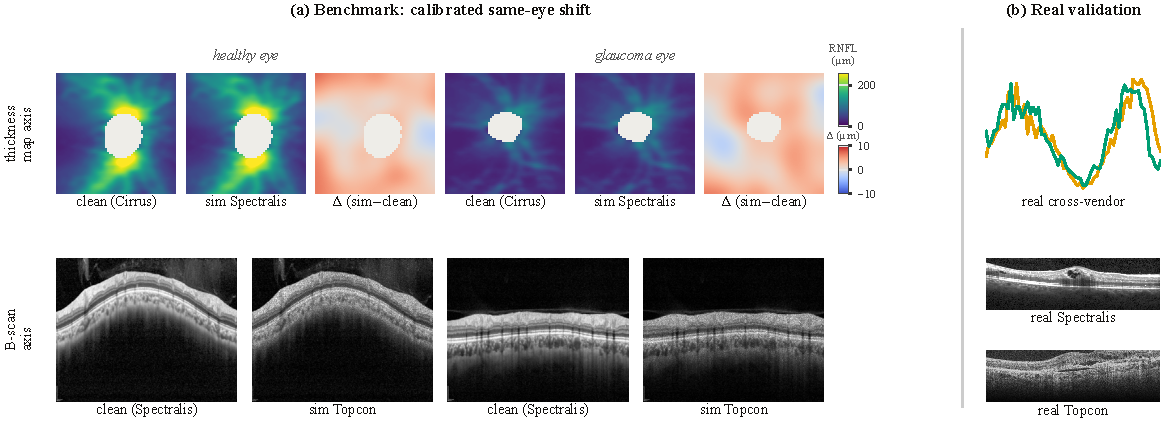
\includegraphics[width=\linewidth]{figures/fig1_overview.pdf}
  \caption{\textbf{The benchmark and its real-data validation.} \textbf{(a)}~The calibrated same-eye shift on
  best-by-eye exemplars. One clear healthy and one clear glaucomatous eye are each shown clean $\rightarrow$ shifted
  on both axes: thickness maps (Harvard-GDP Cirrus, Warner-calibrated Cirrus$\rightarrow$Spectralis; viridis,
  brighter = thicker RNFL) and circumpapillary B-scans (GLEAM Spectralis $\rightarrow$ simulated Topcon). The shift
  is small by design, so each clean/shifted map pair is followed by a difference panel (sim $-$ clean, coolwarm, on a
  shared $\pm10\,\mu$m scale spanning the calibrated LoA), with the largest deviations in the superior and inferior nerve-fiber bundles, where the
  calibrated cross-scanner shift is widest (\S\ref{app:validity}). This is one representative per-eye realization; the
  benchmark applies an independent calibrated shift to every eye. Each reader sees clean and shifted versions of the same eyes, so scanner
  is not confounded with cohort. \textbf{(b)}~Real data corroborating the shift: cross-vendor cpRNFL (circumpapillary RNFL)
  profiles from GLEAM Spectralis and GOALS Topcon agree in shape, and RETOUCH Spectralis/Topcon
  macular B-scans calibrate the per-vendor speckle of the B-scan axis.}
  \label{fig:overview}
\end{figure}

\paragraph{Common-ground harness.} Every reader (a map-reader, an FM linear probe (LP) or fine-tune, or a prompted
VLM) produces the same output: a per-eye glaucoma probability. We score each on paired clean$\rightarrow$shifted
degradation over the same test eyes under the same shared-seed shift, with eye-level percentile-bootstrap 95\% CIs
(2000 resamples; the eye is the unit of analysis; seed-0 split). Each result is labeled by its input
representation, and we never cross-rank across axes.

\paragraph{Two calibrated axes} (Fig.~\ref{fig:overview}; validity in App.~\ref{app:validity}). The two axes span the
three most common OCT vendors (Cirrus, Spectralis, Topcon), which are known not to be interchangeable
\citep{buchser2012}. Each source vendor is fixed by its dataset; we take as the target the pair with a
published calibration anchor (Cirrus$\rightarrow$Spectralis for the thickness map, Spectralis$\rightarrow$Topcon for
the B-scan; App.~\ref{app:validity}). The two axes therefore span two vendor pairs and two shift mechanisms, and the
failure modes recur across both. The two axes are also the two input representations: the color thickness-map and the
raw B-scan, so F2's representation contrast and the two shift axes are the same two settings. \emph{Thickness-map
axis}: Harvard-GDP Cirrus RNFLT maps \citep{luo2023harvardgdp} with labels
($n{=}300$ test, 46\% glaucoma). The shift has three calibrated components: a per-eye bias and limit of agreement
($+1.94\,\mu$m, $\pm7.68\,\mu$m, Warner-calibrated \citep{warner2011loa, blandaltman1986}); a superior/inferior-wider
sector profile from scan-circle centration \citep{cheung2009scancircle}; and a spatially-correlated texture from OCT
segmentation differences \citep{mansberger2017segerrors}. All are matched to real cross-vendor data
(\S\ref{app:validity}). \emph{B-scan axis}: GLEAM \emph{circumpapillary} Spectralis
B-scans \citep{gleam2026} with clinical labels ($n{=}360$ test, 49\% glaucoma). The shift is a Spectralis$\rightarrow$Topcon
appearance stress: a frame-averaging change, injected multiplicative-Gamma speckle, and contrast dimming
\citep{schmitt1999speckle}. Its direction and magnitude are calibrated from real per-vendor RETOUCH macular display
speckle \citep{bogunovic2019retouch}. This axis tests tolerance to appearance changes: its magnitude is
speckle-matched, not bounded by a measured cross-scanner LoA, which would require same-eye disc-OCT on two scanners
that no public dataset provides.

\paragraph{Decision-level metrics.} We report discrimination, decision, and calibration reads; clean AUC, decision-flip, and
$\Delta$sens@spec carry eye-level 95\% bootstrap CIs, and the remaining reads are point estimates. \emph{Discrimination:} clean AUC and $\Delta$AUC (signed clean$-$shift). \emph{Decision:}
decision-\emph{flip} \citep{hendrycks2019corruptions}, the fraction of eyes whose decision (refer / do-not-refer)
changes under the shift; $\Delta$sens@spec, the clean$-$shift change in sensitivity at the operating point; and
\emph{spec@shift}, the specificity actually realized under the shift, which flags a reader that keeps its flip low
only by collapsing specificity. \emph{Calibration:} ECE and $\Delta$ECE \citep{guo2017calibration} over 10
equal-width bins, and the net calibration error (NCE), a signed calibration error \citep{groot2024overconfidence}:
mean predicted-class confidence minus accuracy, so $+$ $=$ overconfident. The operating point is a single threshold fixing 90\% specificity
on clean negatives, applied to shifted scores; fixing it on the clean data makes clean specificity slightly
optimistic, but equally for every reader, so comparisons are unaffected. Because a recalibrating shift leaves
$\Delta$AUC$\approx$0 while the decision flips, it is flip, $\Delta$sens, and spec@shift, not $\Delta$AUC, that reveal the failure.

\paragraph{Readers.} \emph{Frontier closed VLMs} (three developers): Gemini (2.5 Flash, 2.5 Pro, 3.6 Flash),
GPT-5.6 Sol, and Claude Opus~5, zero- and few-shot (k{=}6, single greedy sample; temperature-0 where the API accepts
it, App.~\ref{app:setup}), on both the raw B-scan and a color
thickness-map render. \emph{Open-weights
and specialist VLMs} (self-hosted): Qwen3-VL-8B \citep{qwen3vl2025} and MedGemma-1.5-4B \citep{medgemma15_2026}, same protocol. Elicitation is verbalized
probability \citep{tian2023calibration}: each model states its probability of glaucoma in words rather than reading
it from output logits, the one score common to every vendor, since the closed models expose no
logprobs. \emph{OCT and generic FMs:} RETFound \citep{zhou2023retfound} and MIRAGE \citep{morano2025mirage} against DINOv2 \citep{oquab2023dinov2}, LP and fine-tune.
\emph{ImageNet CNN model-size sweep:} ResNet-50 and ConvNeXt-T/B/L (26M$\rightarrow$197M), frozen probe and
per-architecture fine-tune. \emph{From-scratch:} a 98k-parameter SmallCNN trained end-to-end on each axis.

% ======================================================================================
\section{Experiments and findings}
\label{sec:findings}

We score 29 configurations on the B-scan axis and 25 on the thickness-map axis (the OCT-specific B-scan FMs are not run on map
renders; setup and model/dataset cards in App.~\ref{app:setup}--\ref{app:datasets}). Each finding below states one
claim and gives its eye-level bootstrap-CI evidence; cross-configuration comparisons are descriptive and uncorrected.
Table~\ref{tab:main} lists the headline configurations. Figs.~\ref{fig:stability}--\ref{fig:mechanism} give the
reliability landscape and the shift mechanism.

\begin{table}[t]
  \centering
  \caption{\textbf{Headline configurations, both axes} (calibrated shift, eye-level bootstrap 95\% CIs). Columns: clean AUC,
  decision-\emph{flip}, $\Delta$sens@spec (signed clean$-$shift), clean ECE, net calibration error (NCE) and
  $\Delta$AUC. Lower flip, $|\Delta\text{sens}|$, ECE and $|\Delta\text{AUC}|$ are better. \textbf{Bold} is the best
  AUC, flip and ECE per column among readers with useful discrimination (clean AUC $\ge 0.70$); a near-chance reader
  can post a trivially low flip, so flip is read together with AUC. NCE is a signed calibration error
  \citep{groot2024overconfidence} (mean predicted-class confidence minus accuracy; $+$ $=$ overconfident); $\Delta$sens,
  NCE and $\Delta$AUC are signed diagnostics ($\approx$0 ideal) and are not bolded. The ImageNet-CNN row is the best
  per axis; the from-scratch SmallCNN is trained end-to-end on each axis and never sees the test shift. VLMs are
  prompted (\textit{fs} = few-shot). Full per-axis tables (B-scan 29 configurations, map 25), with realized spec@shift
  and flip/$\Delta$sens CIs, are in App.~\ref{app:fulltables}.}
  \label{tab:main}
  \small
  \renewcommand{\arraystretch}{0.9}
  \setlength{\tabcolsep}{3pt}
  \begin{tabular}{llcccccc}
    \toprule
    Reader & Class & AUC \ci{95\%}{CI} & Flip$\downarrow$ & $\Delta$sens & ECE$\downarrow$ & NCE & $\Delta$AUC \\
    \midrule
    \multicolumn{8}{l}{\textit{\textbf{B-scan axis}} \quad Spectralis\,$\rightarrow$\,Topcon, $n{=}360$ eyes} \\
    \midrule
    DINOv2\,$\cdot$\,FT       & generic FM     & \textbf{0.88} \ci{0.84}{0.91} & \textbf{0.09} & $+0.08$ & 0.05 & $-0.00$ & $+0.01$ \\
    RETFound\,$\cdot$\,FT     & OCT FM         & 0.85 \ci{0.80}{0.89}          & 0.14 & $-0.09$ & 0.07 & $+0.07$ & $-0.01$ \\
    MIRAGE\,$\cdot$\,LP       & OCT FM         & 0.70 \ci{0.65}{0.76}          & 0.47 & $-0.72$ & \textbf{0.04} & $-0.02$ & $+0.04$ \\
    ConvNeXt-B\,$\cdot$\,LP   & ImageNet CNN   & 0.83 \ci{0.78}{0.87}          & 0.11 & $+0.07$ & 0.07 & $+0.03$ & $+0.04$ \\
    SmallCNN (98k)           & scratch CNN    & 0.79 \ci{0.74}{0.83}          & 0.27 & $-0.32$ & \textbf{0.04} & $-0.04$ & $+0.02$ \\
    Gemini 3.6 Flash\,\textit{fs}  & frontier VLM   & 0.69 \ci{0.64}{0.74}          & 0.15 & $+0.01$ & 0.26 & $+0.26$ & $-0.00$ \\
    GPT-5.6 Sol\,\textit{fs}     & frontier VLM   & 0.67 \ci{0.61}{0.73}          & 0.24 & $+0.11$ & 0.23 & $+0.23$ & $-0.01$ \\
    Claude Opus~5\,\textit{fs}& frontier VLM  & 0.67 \ci{0.62}{0.73}          & 0.18 & $+0.05$ & 0.16 & $+0.13$ & $+0.03$ \\
    Qwen3-VL-8B\,\textit{fs} & open VLM       & 0.54 \ci{0.49}{0.58}          & 0.02 & $+0.00$ & 0.38 & $+0.38$ & $+0.00$ \\
    MedGemma-1.5-4B\,\textit{fs}    & specialist VLM & 0.49 \ci{0.43}{0.54}          & 0.00 & $+0.03$ & 0.42 & $+0.42$ & $-0.04$ \\
    \midrule
    \multicolumn{8}{l}{\textit{\textbf{Thickness-map axis}} \quad Cirrus\,$\rightarrow$\,Spectralis, $n{=}300$ eyes} \\
    \midrule
    DINOv2\,$\cdot$\,FT       & generic FM     & \textbf{0.88} \ci{0.83}{0.91} & 0.04 & $+0.01$ & 0.09 & $-0.02$ & $+0.00$ \\
    ConvNeXt-L\,$\cdot$\,FT   & ImageNet CNN   & 0.87 \ci{0.83}{0.91}          & \textbf{0.02} & $+0.01$ & \textbf{0.07} & $-0.04$ & $+0.00$ \\
    SmallCNN (98k)           & scratch CNN    & 0.85 \ci{0.80}{0.89}          & \textbf{0.02} & $+0.00$ & 0.12 & $+0.03$ & $-0.01$ \\
    GPT-5.6 Sol\,\textit{fs}     & frontier VLM   & 0.84 \ci{0.79}{0.88}          & 0.09 & $+0.02$ & 0.11 & $+0.11$ & $-0.00$ \\
    Gemini 3.6 Flash\,\textit{fs}  & frontier VLM   & 0.84 \ci{0.79}{0.88}          & 0.05 & $+0.06$ & 0.15 & $+0.13$ & $+0.02$ \\
    Claude Opus~5\,\textit{fs}& frontier VLM  & 0.83 \ci{0.78}{0.88}          & 0.09 & $+0.03$ & \textbf{0.07} & $+0.01$ & $-0.00$ \\
    Qwen3-VL-8B\,\textit{fs} & open VLM       & 0.59 \ci{0.55}{0.62}          & 0.05 & $+0.00$ & 0.36 & $+0.36$ & $+0.02$ \\
    MedGemma-1.5-4B\,\textit{fs}    & specialist VLM & 0.55 \ci{0.48}{0.61}          & 0.03 & $+0.00$ & 0.30 & $+0.30$ & $+0.02$ \\
    \bottomrule
  \end{tabular}
\end{table}


\begin{figure}[t]
  \centering
  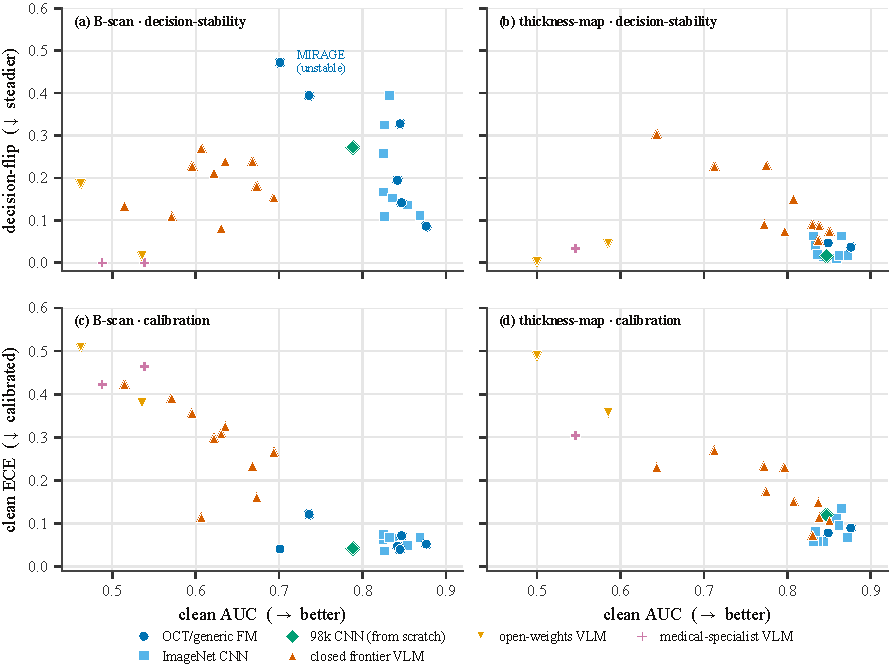
\includegraphics[width=0.9\linewidth]{figures/fig2_stability.pdf}
  \caption{\textbf{Reliability landscape.} Every reader on clean AUC against two reliability metrics,
  \emph{decision-stability} (decision-flip, top row) and \emph{calibration} (clean ECE, bottom row), for the
  B-scan (left) and thickness-map (right) axes. Color and marker encode reader class. Frontier VLMs are
  unstable and overconfident on the raw B-scan (a,c) but recover on the thickness map (b,d); the small open and
  specialist VLMs are near chance on both axes. A $\Delta$AUC$\approx$0 can hide large decision-flips (MIRAGE, panel a), and the
  98k-parameter from-scratch CNN (green diamond) is among the steadiest readers on the thickness-map axis
  (b), CI-tied with the best CNNs, though not steady on the raw B-scan (a).}
  \label{fig:stability}
\end{figure}

\paragraph{F1: prompted frontier VLMs are the weakest and most overconfident above-chance readers, across three developers.}
Among the readers above near-chance, the prompted frontier VLMs rank last. On the raw B-scan, even the best frontier
VLM only matches the weakest specialist's discrimination (MIRAGE\,$\cdot$\,LP, AUC \num{0.70}): Gemini 3.6 Flash few-shot AUC
\num{0.69} \ci{0.64}{0.74}, GPT-5.6 Sol \num{0.67} \ci{0.61}{0.73}, and Claude Opus~5 \num{0.61}/\num{0.67}
(zero/few-shot). The Gemini and GPT configurations are also badly overconfident: their clean (pre-shift) ECE is
\num{0.23}--\num{0.42}, roughly 5--10$\times$ the best FM's \num{0.04}, and their net calibration
error is also large and positive (\num{0.23}--\num{0.42}; per configuration in Table~\ref{tab:main} and
App.~\ref{app:fulltables}), so the miscalibration is overconfidence, not two-sided noise. The gap is not a binning
artifact: it holds under a strictly proper score (Brier) and adaptive-bin ECE, not just fixed-bin ECE
(App.~\ref{app:fulltables}), matches \citet{groot2024overconfidence, xia2024cares}, and is the VLM/FM split in
Fig.~\ref{fig:stability}c. Few-shot lifts discrimination with mixed calibration effect, whereas neither a larger model
nor a higher tier helps (the higher-tier Gemini 2.5 Pro is the worst frontier zero-shot, AUC \num{0.51}). Calibration
is vendor-dependent, with Claude Opus~5 a markedly better exception (ECE \num{0.11}--\num{0.16}). The weakness deepens as models shrink: the open-weights
Qwen3-VL-8B and the specialist MedGemma-1.5-4B are near chance on both axes (AUC \num{0.41}--\num{0.59}) with the highest
ECE (up to \num{0.51}), so neither open weights nor medical-specialist pretraining rescues the decision (the
small-model elicitation caveat in \S\ref{sec:discussion} applies).

\paragraph{F2: general-purpose VLMs read the thickness map, not the raw B-scan.}
On the thickness-map task the same models reach the strong generic-FM/CNN readers' level (DINOv2, ConvNeXt): Gemini
3.6 Flash \num{0.84}, GPT-5.6 Sol \num{0.84} \ci{0.79}{0.88}, and Claude Opus~5 \num{0.83} \ci{0.78}{0.88}. Discrimination,
calibration (ECE roughly halved), and stability (flip dropping) recover together, well above their raw-B-scan level
and across all three developers (per-VLM detail in App.~\ref{app:grounding}). The lift holds even zero-shot (GPT-5.6 Sol \num{0.77} vs.\ \num{0.63}; Claude Opus~5
\num{0.61}$\rightarrow$\num{0.85}), so it is not few-shot memorization, but it needs a capable base: the small open
VLMs do not recover (Qwen3-VL-8B \num{0.50}--\num{0.59}, MedGemma-1.5-4B \num{0.41}--\num{0.55}). The gap is specific to
general-purpose VLMs on the raw B-scan, where reading RNFL requires the implicit segmentation an OCT-trained model
performs while a color thickness map presents thinning directly. A thickness map is not intrinsically a better input
(trained models read glaucoma from raw OCT at least as well \citep{maetschke2019}), and because the two axes use
different datasets this comparison is confounded (\S\ref{sec:discussion}).

\begin{figure}[t]
  \centering
  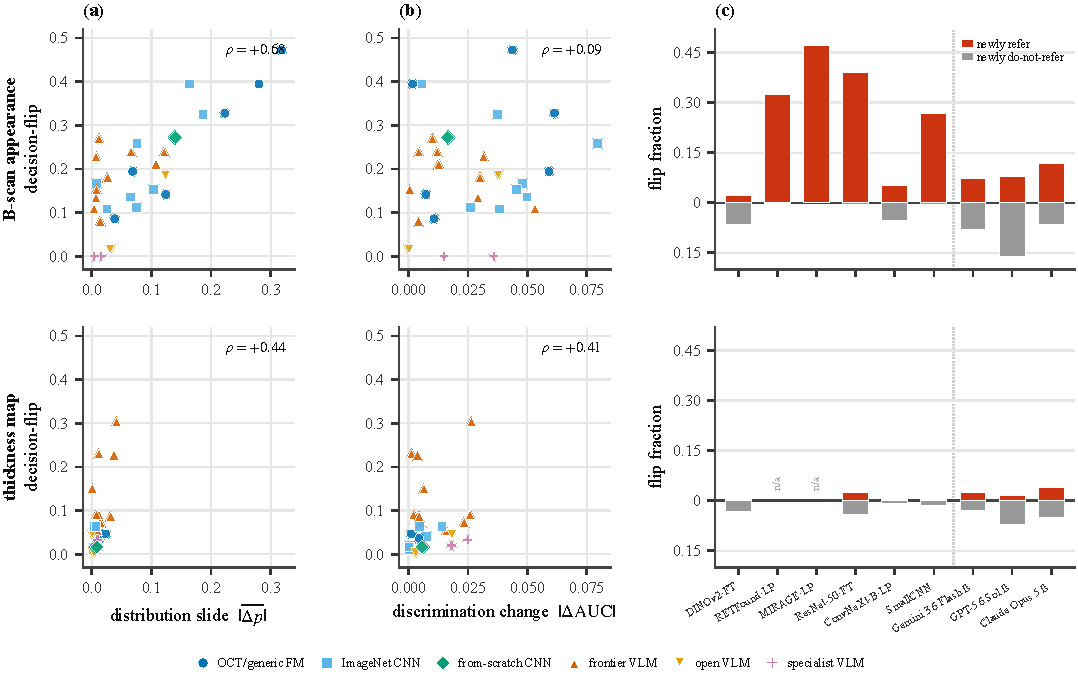
\includegraphics[width=\linewidth]{figures/fig3_mechanism.pdf}
  \caption{\textbf{Decision-flip comes from the score distribution moving, not from a change in discrimination.}
  One row per shift axis (top: B-scan appearance; bottom: thickness map), with matched limits. Across all 29 B-scan
  readers, decision-flip is uncorrelated with the discrimination change $|\Delta\text{AUC}|$ (\textbf{b},
  $\rho{=}0.09$) and rises with the net directional slide $|\overline{\Delta p}|$ (\textbf{a}, $\rho{=}0.68$); readers
  well above the (\textbf{a}) trend (real flip at near-zero net slide) move two-sidedly, and flip tracks the mean
  absolute per-eye movement mean\,$|\Delta p|$ (not plotted) even more tightly ($\rho{=}0.88$). A reader can flip many decisions with its AUC intact. On the
  thickness-map axis (bottom) slide, $|\Delta\text{AUC}|$, and flip are all small.
  \textbf{(c)}~Decision-flip split into newly-``refer'' (over-referral, red) and newly-``do-not-refer'' (grey), for
  representative readers per class plus the frontier VLMs (few-shot; the dotted line separates non-VLM from VLM). The
  appearance-sensitive readers (the OCT FMs MIRAGE\,$\cdot$\,LP and RETFound\,$\cdot$\,LP, the ImageNet
  ResNet-50\,$\cdot$\,FT, and the from-scratch SmallCNN) over-refer almost one-directionally, whereas the generic
  DINOv2\,$\cdot$\,FT and ConvNeXt-B\,$\cdot$\,LP stay robust (small, two-sided). The VLMs flip in
  \emph{model-specific} directions (GPT-5.6 Sol toward do-not-refer, Claude Opus~5 toward refer, Gemini 3.6 Flash either way). The map row (bottom) is
  likewise near-flat for every reader, and the OCT-specific FMs, not run on maps, are marked n/a. Markers in (a,b)
  encode reader class (shared legend).}
  \label{fig:mechanism}
\end{figure}

\paragraph{F3: a scanner change can break the decision while discrimination holds.}
Decision-flip is unrelated to discrimination: across all \num{29} B-scan readers $|\Delta\text{AUC}|\le\num{0.08}$
(about half within \num{0.03}), yet decision-flip spans \num{0.00}--\num{0.47} and shifted specificity \num{0.07}--\num{1.00},
and flip is uncorrelated with $\Delta$AUC (Spearman \num{0.09}). Flip is instead a threshold effect: it rises with the
mean absolute per-eye movement mean\,$|\Delta p|$ (Spearman \num{0.88}; movement $\Delta p =
p_{\text{shift}}-p_{\text{clean}}$) more tightly than with the net directional slide $|\overline{\Delta p}|$
(\num{0.68}; Fig.~\ref{fig:mechanism}a,b), because some readers move their scores two-sidedly and flip without a net
direction. What matters for safety is the direction of the crossings. In the appearance-sensitive readers (the OCT
FMs, the fine-tuned ImageNet CNNs, and the from-scratch SmallCNN) the added speckle pushes scores up, so essentially
every threshold crossing is toward ``refer'' and specificity collapses; the up-shift largely preserves the ordering
of eyes, so AUC holds. MIRAGE\,$\cdot$\,LP is the extreme (all \num{170} flips up, specificity \num{0.07}), with
RETFound\,$\cdot$\,LP ($117/118$ up) and ResNet-50\,$\cdot$\,FT ($140/142$ up) the same, and \num{18}/\num{29} readers
net-shift toward refer (OCT FMs mean $\overline{\Delta p}=+0.24$). This is over-referral, not lost sensitivity
(Fig.~\ref{fig:mechanism}c), and it concentrates on healthy eyes (MIRAGE\,$\cdot$\,LP flips \num{62}\% of healthy
vs.\ \num{28}\% of moderate-to-advanced; no disparity across demographics, underpowered subgroups,
App.~\ref{app:subgroups}). The frontier VLMs and the broadly-pretrained DINOv2 show no such systematic over-referral:
the VLMs flip in model-specific directions (GPT-5.6 Sol toward do-not-refer, Claude Opus~5 toward refer, Gemini 3.6 Flash
either way; flip \num{0.15}--\num{0.24}), and DINOv2 resists ($\overline{\Delta p}=-0.04$), the steadiest capable
reader (flip \num{0.09}). Either way AUC-only evaluation misses the flip while the decision-level metrics expose it.
The thickness-map axis is far more stable ($|\Delta\text{AUC}|\le\num{0.03}$, flip $\le\num{0.31}$).

\paragraph{F4: stability does not track model size; representation and pretraining breadth win.}
Frozen LP clean AUC is unchanged across 26M$\rightarrow$197M (map \num{0.83}--\num{0.84}, B-scan
\num{0.82}--\num{0.83}; CIs overlap), and the largest model is steadiest on neither axis; the color thickness-map is
robust at every size while the raw B-scan is not. Generic DINOv2 is the steadiest and best-discriminating (B-scan
LP$\rightarrow$FT flip \num{0.19}$\rightarrow$\num{0.09}), whereas OCT-specific MIRAGE is weakest (AUC \num{0.70}, flip
\num{0.47}); fine-tuning rescues the other OCT FM (RETFound\,$\cdot$\,FT flip \num{0.14}, AUC \num{0.85}), so the
weakness is MIRAGE-specific, not intrinsic to OCT pretraining, though fine-tuning is no universal fix and can itself
distort features under shift \citep{kumar2022finetuning}. The clearest case is a from-scratch 98k-parameter SmallCNN, trained
end-to-end on the thickness map and never exposed to the test shift: it flips just \num{0.02} \ci{0.00}{0.03} (net
calibration error \num{0.03}), CI-tied with the best ImageNet CNNs and steadier than the 300M DINOv2 (flip
\num{0.04}) at $\sim$900--3000$\times$ fewer parameters, so its stability is a genuine out-of-distribution result
from the compact, task-trained representation, not model size.

% ======================================================================================
\section{Discussion and limitations}
\label{sec:discussion}

\paragraph{What this means for deployment.} Used in a glaucoma-diagnosis pipeline today, a prompted generalist
VLM reading raw B-scans is the least safe above-chance reader: below the specialist FMs and markedly overconfident. But a strong FM or CNN fails differently: it holds its AUC under a
scanner change while its decisions flip, so it passes single-scanner validation and then fails in the field. Where that flip is a specificity collapse, it over-refers the healthy
majority of a screening population (\S\ref{sec:findings}), the costliest place for false referrals. Two things follow. First, this is a decision failure,
not a calibration one: calibration is already poor before any shift and does not significantly worsen under it
($\Delta$ECE CI includes 0), and post-hoc temperature scaling \citep{guo2017calibration} removes most of the clean VLM
ECE (App.~\ref{app:reliability}) yet, being monotonic, leaves the decision-flip unchanged. Second, re-thresholding cannot undo this score movement at
deployment, where no labeled data from the incoming scanner exist, so the remedy is to select readers whose decisions
stay put. The recommendation is concrete: validate a diagnostic reader at its operating point, with calibration and
under a scanner shift, not on single-scanner AUC; our benchmark is that check, and a candidate that flips a quarter of
decisions under a calibrated same-eye shift is unsafe however high its AUC.

\paragraph{What to engineer, and why.} The failure is not fundamental to VLMs. The same models recover to the strong
generic-FM/CNN level once the RNFL is rendered as a readable color thickness map (a cross-dataset contrast; see
\emph{Limitations}). What helps is the input
representation, not model size, vendor, or a ``medical-specialist'' label. The B-scan failure is an appearance
sensitivity, consistent with the added speckle and dimmed contrast being read as RNFL thinning: appearance-keyed readers
(the OCT-specific FMs and fine-tuned CNNs) raise their glaucoma score and over-refer while the broadly-pretrained
generic FM resists (F3--F4); the small open and specialist models recover on neither, so it is an interaction of input format and
capability. Robustness tracks representation and pretraining breadth, not model size: a 98k-parameter task-trained CNN is among
the steadiest readers at $\sim$900--3000$\times$ fewer parameters than the FMs. For practitioners: engineer the input
representation and a compact, task-specific encoder, and require decision stability, not model size, before deployment.

\paragraph{Limitations.} \emph{The same-eye shift is synthetic}: no public same-eye cross-scanner labeled disc-OCT
exists, so we calibrate the shift to published cross-scanner LoA (map) and real per-vendor speckle (appearance) and
keep four datasets real; a real same-eye cross-scanner set is the natural extension. \emph{Elicitation and
calibration are conservative}: VLMs are queried with a single greedy verbalized-probability sample, so the reported
VLM ECE is an upper estimate of overconfidence ($N$-sample, prompt-paraphrase passes are future work); the smallest
open models collapse to a constant (Qwen3-VL-8B on the map), so a boolean-verdict elicitation may be fairer.
\emph{The B-scan-vs-thickness-map comparison (F2) is cross-dataset}: the two axes differ in
dataset, vendor, and labels, so F2 confounds input representation with dataset difficulty and possible
contamination; we read it as reader-specific (\S\ref{sec:findings}), not as evidence a map is better in general.
\emph{Subgroups}: instability is broadly uniform across disease severity and demographics
(App.~\ref{app:subgroups}), but the subgroups are underpowered and image quality is unrecorded, so a definitive
fairness audit needs richer metadata. \emph{Scope}: two axes, never cross-ranked; broader vendor-pair coverage and
extending decision stability to longitudinal progression monitoring are the natural next steps.

% ======================================================================================
\section{Conclusion}
\label{sec:conclusion}

A scanner change can break a glaucoma-OCT reader's decision while its AUC looks unchanged; reliability tracks input
representation and pretraining breadth, not model size. We release our de-confounded, decision-level,
calibration-aware benchmark (four real datasets, only the scanner shift synthesized) as a reusable check, so a
reader's decision stability under a scanner change can be validated before it reaches patients.


\bibliographystyle{plainnat}
\bibliography{references}

\newpage
\appendix
% ======================================================================================
%  Appendix
% ======================================================================================
\section{Experimental setup}
\label{app:setup}

\paragraph{Encoders.} Foundation models (RETFound, MIRAGE, DINOv2) and CNNs (ResNet-50, ConvNeXt-T/B/L, the
98k-parameter SmallCNN) are frozen feature extractors with a linear head, or fine-tuned end-to-end (``FT'').
\emph{Linear probe:} \texttt{StandardScaler} + $\ell_2$ logistic regression, \texttt{LogisticRegressionCV}
($C\in\{0.01,0.05,0.2,1.0\}$, 3-fold, ROC-AUC, \texttt{max\_iter}=5000; small-$n$ fallback $C{=}0.05$), fit on clean
training eyes (seed-0). Features: DINOv2 = \texttt{[CLS]}\,$\oplus$\,mean patch tokens (registers excluded) at
$224^2$; RETFound = global-avg-pool + \texttt{fc\_norm} at $224^2$ (ImageNet normalization); MIRAGE = encoder last
token at native $512^2$ (unit-scaled, not ImageNet-normed); ResNet/ConvNeXt = global-avg-pool. \emph{Fine-tune:}
AdamW (weight decay 0.05), 50 epochs, batch 32, layer-wise LR decay (ConvNeXt 0.9 / ResNet 1.0 / ViT 0.65),
base-LR $5\times10^{-4}$/$10^{-3}$/$5\times10^{-3}$ linearly scaled by batch, warmup then cosine to $10^{-6}$,
class-weighted cross-entropy with label-smoothing 0.1, \texttt{RandomResizedCrop}(0.5--1.0)+HFlip+RandomErasing(0.25)
at $224^2$, mixed precision, early stop (patience 12) on validation AUC. \emph{SmallCNN} ($\sim$98k params):
four \texttt{Conv}$3{\times}3$--GroupNorm--ReLU--MaxPool blocks (16/32/64/128) $\rightarrow$ global-avg-pool
$\rightarrow$ linear logit; Adam ($10^{-3}$, wd $10^{-4}$), class-weighted BCE. It is trained end-to-end from scratch
on each scored axis (GLEAM B-scans; Harvard-GDP thickness maps), on the same seed-0 split as the other readers. It is
never exposed to the test shift.

\paragraph{VLMs.} All seven VLMs receive byte-identical eyes, shifts (per-eye seeds $3000{+}e$, $4000{+}e$), few-shot
exemplars (seed $+11$) and prompts from a single shared axis builder, are queried greedily (one
sample) for a verbalized probability \citep{tian2023calibration}, and are thresholded at the clean-data
90\%-specificity operating point. Exact model IDs and inference settings are in Table~\ref{tab:models}. The verbatim
prompts, few-shot construction and probability parsing are in App.~\ref{app:prompts}.

\paragraph{Statistics.} Confidence intervals are eye-level percentile bootstraps (2000 resamples; the eye is the
resampling unit) \citep{diciccio1996bootstrap}. ECE uses 10 equal-width confidence bins \citep{guo2017calibration}. The operating point (target specificity 0.90) is fixed on
clean negatives and reused on shifted scores; $\Delta$sens@spec and spec@shift are read there, while decision-flip
is the change in the fixed $0.5$ clinical call (refer / do-not-refer). Both capture decision movement at a
deployed threshold. Sample sizes: $n{=}360$ eyes (B-scan axis), $n{=}300$ eyes (thickness-map
axis).

\paragraph{Compute.} The open-weights VLMs and all fine-tuning run on a single Colab GPU (A100-40GB or L4), bf16,
\texttt{device\_map=auto}, batched greedy generation. The closed API configurations (Gemini, GPT-5.6 Sol, Claude) are CPU-only
clients. Reproducing the tables and figures from the released per-eye outputs requires no GPU.

\section{Prompts and elicitation}
\label{app:prompts}

Elicitation is a single verbalized referral probability per eye \citep{tian2023calibration}, the score common to
every vendor, since the closed models expose no logprobs. Prompts are byte-identical across models on a given axis.

\paragraph{B-scan axis.} System: \emph{``You are grading circumpapillary OCT B-scans for glaucoma. Each
image is a cross-sectional retinal scan taken in a ring around the optic nerve head. Glaucoma shows as thinning/loss
of the retinal nerve fibre layer (RNFL) and neuroretinal rim.''} Query: \emph{``Now assess THIS new B-scan. Return
JSON: \texttt{glaucoma\_referral\_probability} (0--1, your calibrated probability that this eye should be referred
for glaucoma), \texttt{rationale} (one short sentence).''}

\paragraph{Thickness-map axis.} System: \emph{``You are grading en-face retinal nerve fibre layer (RNFL) THICKNESS
MAPS for glaucoma. Each image is a colour-coded map of RNFL thickness around the optic disc: warm colours = THICK,
cool colours = THIN. Glaucoma shows as THINNING---loss of the bright superior and inferior nerve-fibre bundles (the
`double-hump'), a wedge defect or diffuse darkening.''} Query: as above with ``RNFL thickness map''.

\paragraph{Few-shot.} $k{=}6$ labeled exemplars, drawn only from the training pool (leakage guard), balanced:
B-scan axis severity-graded (3 healthy + one each early/moderate/advanced); map axis binary (3 glaucoma + 3
healthy). Selection RNG is \texttt{seed}$+11$ and the exemplar set is identical across models. The few-shot preamble
adds \emph{``Below are LABELLED reference images in this exact format so you can calibrate''}; each exemplar is
captioned with its label before (API/open configurations) or after (Gemini) its image.

\paragraph{Probability parsing.} We read \texttt{glaucoma\_referral\_probability} from the JSON (regex fallback on
the first such field, clipped to $[0,1]$); parse failures are retried (up to 5, exponential backoff) and, only if
still failing, imputed as 0.5 (never cached). Imputation is rare for the frontier configurations but non-negligible
for the small-model configurations that collapse to a near-constant output (e.g.\ Qwen3-VL-8B on the map), where it
biases ECE and AUC toward chance and reinforces the near-chance reading of those configurations. An alternative boolean-verdict schema
maps $p{=}\text{conf}$ if glaucoma else $1{-}\text{conf}$. We use the probability schema throughout for parity.

\begin{table}[t]
  \centering
  \caption{\textbf{Model card.} Exact identifiers, size and inference settings. VLMs are queried $N{=}1$,
  greedily. Reasoning/thinking is enabled where supported (``high''/dynamic). Temperature is omitted for the
  reasoning API models (they reject it) and set to 0 for Gemini.}
  \label{tab:models}
  \small
  \renewcommand{\arraystretch}{0.9}
  \setlength{\tabcolsep}{4pt}
  \begin{tabular}{lll}
    \toprule
    Model & Identifier & Params / settings \\
    \midrule
    \multicolumn{3}{l}{\textit{Vision-language models (prompted)}} \\
    \midrule
    Gemini 2.5 Flash / Pro & \texttt{gemini-2.5-flash}, \texttt{-pro} & temp 0, thinking budget \\
    Gemini 3.6 Flash & \texttt{gemini-3.6-flash} & temp 0, thinking level high \\
    GPT-5.6 Sol & \texttt{gpt-5.6-sol} & reasoning=high, no temp \\
    Claude Opus~5 & \texttt{anthropic/claude-opus-5} & reasoning=high \\
    Qwen3-VL-8B & \texttt{Qwen/Qwen3-VL-8B-Instruct} & 8B, bf16, greedy, 192 tok \\
    MedGemma-1.5-4B & \texttt{google/medgemma-1.5-4b-it} & 4B, bf16, greedy, 192 tok \\
    \midrule
    \multicolumn{3}{l}{\textit{Foundation models / CNNs (frozen probe + fine-tune)}} \\
    \midrule
    DINOv2 (ViT-L/14, reg.) & \texttt{vit\_large\_patch14\_reg4\_dinov2} & $\sim$300M, $224^2$ \\
    RETFound (ViT-L/16) & \texttt{RETFound\_mae\_natureOCT} & $\sim$300M, $224^2$ \\
    MIRAGE-Base (ViT-B) & \texttt{j-morano/MIRAGE-Base} & $\sim$86M, $512^2$ \\
    ResNet-50 & \texttt{resnet50.a1\_in1k} & $\sim$26M \\
    ConvNeXt-T/B/L & \texttt{convnext\_\{t,b,l\}.fb\_in1k} & $\sim$29/88/197M \\
    SmallCNN & from scratch & $\sim$98k \\
    \bottomrule
  \end{tabular}
\end{table}

\section{Datasets}
\label{app:datasets}

All data are public or registered-access research datasets. No new patient data were collected. Splits are
eye-level (one eye per subject where applicable), seed-0, 55/15/30 train/val/test.

\begin{table}[t]
  \centering
  \caption{\textbf{Datasets.} Two are scored (thickness-map and B-scan axes). Two supply the real-data validation
  (cross-vendor anatomy; per-vendor speckle calibration).}
  \label{tab:datasets}
  \small
  \setlength{\tabcolsep}{4pt}
  \resizebox{\linewidth}{!}{%
  \begin{tabular}{lllll}
    \toprule
    Dataset & Role & Modality (region) & $n$ (tr/val/test) & Label / access \\
    \midrule
    Harvard-GDP & thickness-map axis (scored) & Cirrus RNFLT maps $225^2$ (disc) & 550/150/300 & VF-derived; CC BY-NC-ND 4.0 \\
    GLEAM & B-scan axis (scored) & Spectralis circumpapillary B-scans & 660/180/360 & clinical (4-class$\to$binary) \\
    GLEAM\,/\,GOALS & cross-vendor validity & Spectralis + Topcon B-scans $\to$ cpRNFL & 60+60 & single segmenter \citep{driessen2024} \\
    RETOUCH & speckle calibration & Cirrus/Spec/Topcon macular B-scans & $\sim$30/vendor & public challenge \\
    \bottomrule
  \end{tabular}}
\end{table}

Harvard-GDP labels are the \texttt{glaucoma} field per eye \citep{luo2023harvardgdp}; GLEAM is single-center
\citep{gleam2026}, a 4-class severity label binarized to refer/do-not-refer. The cross-vendor validity row is a
\emph{derived measurement}, not a released dataset: we run the device-agnostic ONH-OCT segmenter of
\citet{driessen2024} on GLEAM Spectralis and GOALS Topcon \citep{goals2022} B-scans to produce cpRNFL
profiles, holding the segmentation source constant so the residual cross-vendor difference is imaging plus cohort,
not segmentation. RETOUCH \citep{bogunovic2019retouch} is used only to measure real per-vendor display-speckle
contrast (Cirrus 0.365 $>$ Topcon 0.184 $>$ Spectralis 0.148), not scored. It is macular data, a proxy for the disc. No
public same-eye cross-scanner labeled disc-OCT set exists, which is why the primary shift is a calibrated same-eye
transform (\S\ref{app:validity}).

\section{Reliability diagrams (calibration detail)}
\label{app:reliability}

Fig.~\ref{fig:reliability} shows the ECE gap of \S\ref{sec:findings} (F1) is genuine overconfidence, not a
binning artifact, and systematic across vendors: every frontier-VLM configuration (Gemini, GPT-5.6 Sol, Claude Opus~5,
few-shot) lies below the diagonal (confidence exceeding accuracy) while the OCT/generic FMs and ImageNet CNNs
track it. Vendor-dependence is visible (Gemini furthest below, Claude closest). The FM/CNN per-eye probabilities here
are recomputed from cached encoder features with the same frozen probe (\S\ref{app:setup}), and the recomputed ECE
matches Table~\ref{tab:main}.

\begin{figure}[tbp]
  \centering
  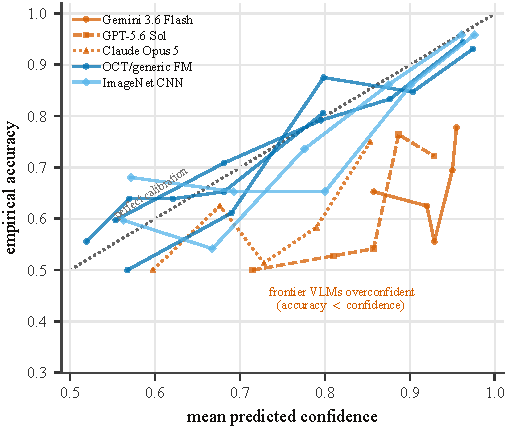
\includegraphics[width=0.55\linewidth]{figures/figA3_reliability.pdf}
  \caption{\textbf{Reliability diagram} (B-scan axis, few-shot), one line per configuration: empirical accuracy vs.\ mean
  predicted confidence in five equal-count bins for readability (dotted = perfect calibration; the ECE metric
  itself uses 10 equal-width bins, \S\ref{app:setup}). Every frontier VLM
  (Gemini 3.6 Flash, GPT-5.6 Sol, Claude Opus~5; one warm color, distinguished by line style) lies below the diagonal
  (overconfident), most for Gemini and least for Claude, whereas the OCT/generic FMs and ImageNet CNNs (cool
  colors) track it (well-calibrated).}
  \label{fig:reliability}
\end{figure}

\paragraph{Net calibration error and post-hoc calibration.} The miscalibration is directional and largely fixable
post hoc, yet the decision failure is not. For each frontier configuration we compute the net calibration error
(NCE), a signed calibration error \citep{groot2024overconfidence}: mean decision-confidence ($\max(p,1{-}p)$) minus
decision accuracy on clean eyes (positive $=$ overconfident; the opposite sign to Groot et al.'s
accuracy$-$confidence convention). (The ECE in Table~\ref{tab:main} is instead the
referral-probability, or positive-class, calibration error; the NCE and the reliability diagram use the
predicted-class confidence $\max(p,1{-}p)$. Both show the frontier VLMs are badly miscalibrated.) The Gemini and GPT
configurations have NCE \num{0.23}--\num{0.42} (few-shot \num{0.23}--\num{0.32}, zero-shot up to \num{0.42}); Claude
Opus~5 is far smaller (\num{0.08}--\num{0.13}), matching the diagram ordering above.
Post-hoc temperature scaling \citep{guo2017calibration} (one scalar fit on a held-out clean half by minimizing NLL)
removes most of the clean ECE (on the held-out clean half: Gemini 3.6 Flash few-shot \num{0.27}$\rightarrow$\num{0.07},
GPT-5.6 Sol \num{0.26}$\rightarrow$\num{0.07}), but, being strictly monotone, it preserves the score ordering and
fixes the $0.5$ decision point, so the decision-flip is exactly unchanged (and the refit 90\%-specificity operating
point selects the same decisions). Calibration is a post-hoc fix; the
scanner-driven decision-flip is not.

\paragraph{Calibration beyond fixed-bin ECE.} Fixed-bin ECE is a biased estimator at $n{\approx}300$--$360$ and
depends on the binning scheme, so we recompute the clean-eye calibration under two complementary reads with different
failure modes: adaptive (equal-count) ECE, which debiases the fixed binning, and the Brier score, a strictly proper
scoring rule with no binning (the proper-score check used under dataset shift by \citet{ovadia2019shift}). Both are
reported for every reader on both axes as extra columns in the full tables (App.~\ref{app:fulltables}). The frontier
VLMs stay worse than every FM/CNN reader on all three reads (fixed-bin ECE, adaptive ECE, and Brier; Claude Opus~5 the
least-overconfident exception), so the overconfidence gap is not an artifact of the ECE binning.

\section{Shift calibration and real-data corroboration}
\label{app:validity}

The synthetic shift is magnitude-tied to the published cross-scanner agreement literature and direction-corroborated
by real data. \emph{Thickness-map axis:} the Cirrus$\rightarrow$Spectralis RNFL offset reproduces
\citet{warner2011loa}'s $+1.94\,\mu$m bias and $\pm7.68\,\mu$m 95\% limits (difference SD $3.92\,\mu$m,
Fig.~\ref{fig:a1}a, a Bland--Altman plot \citep{blandaltman1986}). The per-eye spread is anatomy-coupled, drawn in
quadrature from segmentation, centration, and magnification mechanisms (between-eye SDs $2.8/2.3/1.5\,\mu$m) with
superior/inferior-wider sector gains, so limits widen in the vulnerable sectors (Fig.~\ref{fig:a1}b). The magnitude
is calibrated to Warner's Bland--Altman statistics, and the superior/inferior-wider spatial profile follows the
dominant cross-device error mechanism, scan-circle centration, which perturbs the superior and inferior sectors most
\citep{cheung2009scancircle}; the three mechanism components sum in quadrature to the published SD by construction,
so both the shift magnitude and its sector direction are anchored in measured cross-scanner data and established
optics. The finer within-eye texture is a small mean-zero term for spatially-correlated segmentation differences, which
are largest in the superior and inferior sectors \citep{mansberger2017segerrors}. This smoothness is data-driven: the real cross-vendor cpRNFL difference
(GLEAM Spectralis vs GOALS Topcon) is itself spatially smooth, with $74\%$ of its angular variance
in the lowest five harmonics and a $\sim$$22^{\circ}$ correlation length (roughness $0.79$ vs $1.41$ for white
noise), i.e.\ a low-frequency difference, not per-pixel noise. Being mean-zero, the texture leaves the calibrated
between-eye bias and LoA intact; these are validated directly by the Bland--Altman fit (Fig.~\ref{fig:a1}a) and the
monotone dose--response (Fig.~\ref{fig:a1}c), so Fig.~\ref{fig:overview}'s difference panels illustrate the
calibrated shift rather than assert a per-pixel measurement. Decision-flip and read-drift rise monotonically with dose (Fig.~\ref{fig:a1}c). \emph{B-scan axis:} the
Spectralis$\rightarrow$Topcon stress changes frame-averaging (16$\rightarrow$1 frames), injects a
multiplicative-Gamma speckle field that lifts display-speckle contrast $0.148\rightarrow0.184$ (matched to real
RETOUCH, Fig.~\ref{fig:a2}a), adds near-inert axial blur ($\sqrt{15}\,\mu$m FWHM at $10\,\mu$m/px), and dims
backscatter contrast $\times0.773$. Real cross-vendor cpRNFL corroborates that disc anatomy is vendor-consistent:
with a single segmenter \citep{driessen2024}, cpRNFL profiles from GLEAM Spectralis and GOALS Topcon
\citep{goals2022} B-scans agree in shape ($r\approx0.93$, Fig.~\ref{fig:a2}b). This corroborates that the scanner
perturbs the measurement, not the anatomy; it is a shape agreement, not a claim of scanner-interchangeability.

\begin{figure}[tbp]
  \centering
  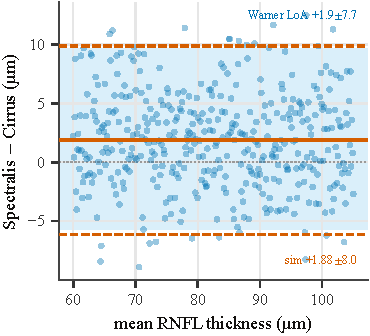
\includegraphics[width=0.32\linewidth]{figures/figA1a_bland_altman.pdf}\hfill
  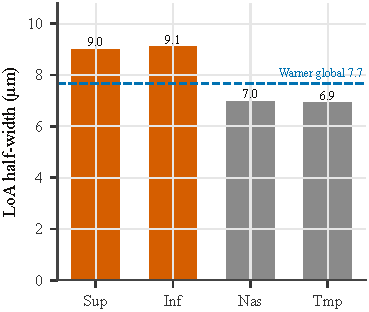
\includegraphics[width=0.32\linewidth]{figures/figA1b_sector_loa.pdf}\hfill
  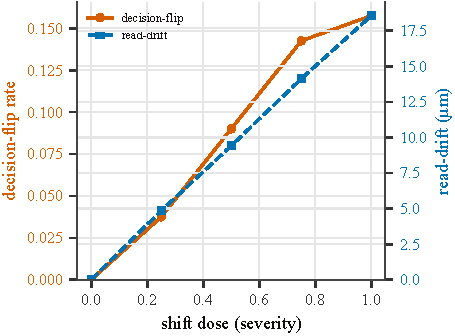
\includegraphics[width=0.32\linewidth]{figures/figA1c_dose_response.pdf}
  \caption{\textbf{Thickness-map shift is LoA-calibrated.} (a)~Bland--Altman of the synthetic per-eye differences
  against Warner's published 95\% limits (band); (b)~limits widen in the superior/inferior sectors;
  (c)~decision-flip and read-drift rise monotonically with shift dose, a graded axis rather than a cliff.}
  \label{fig:a1}
\end{figure}

\begin{figure}[tbp]
  \centering
  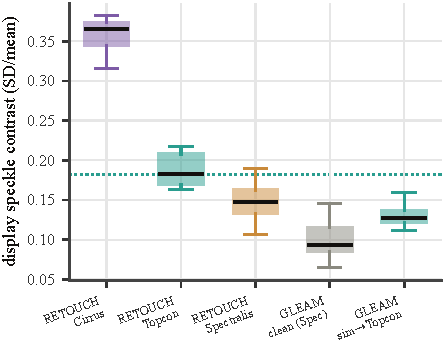
\includegraphics[width=0.44\linewidth]{figures/figA2a_speckle.pdf}\hfill
  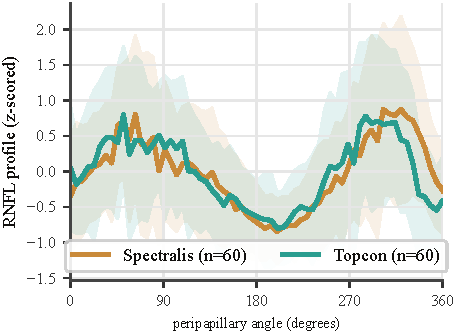
\includegraphics[width=0.44\linewidth]{figures/figA2b_crossvendor.pdf}
  \caption{\textbf{Appearance/anatomy validity.} (a)~Real per-vendor RETOUCH display speckle (Cirrus $>$ Topcon $>$
  Spectralis) validates the frame-averaging direction and the calibrated sim moves GLEAM toward Topcon;
  (b)~real cross-vendor cpRNFL: GLEAM Spectralis vs.\ GOALS Topcon profiles (single segmenter) agree in shape
  ($r\approx0.93$; shape only, not device-interchangeability).}
  \label{fig:a2}
\end{figure}

\section{Thickness-map vs.\ raw-B-scan reading, per VLM (F2)}
\label{app:grounding}
Fig.~\ref{fig:grounding} details F2. Rendering the same eye as a color thickness map instead of a raw B-scan raises
each stronger frontier VLM into the non-VLM reader band on discrimination and pulls it down on ECE and decision-flip
together, while the small open/specialist VLMs do not recover. This is a cross-dataset comparison (the two axes use
different datasets, vendors and label sources), so we read it as reader-specific, not as evidence that a thickness
map is intrinsically a better input (\S\ref{sec:discussion}).

\begin{figure}[tbp]
  \centering
  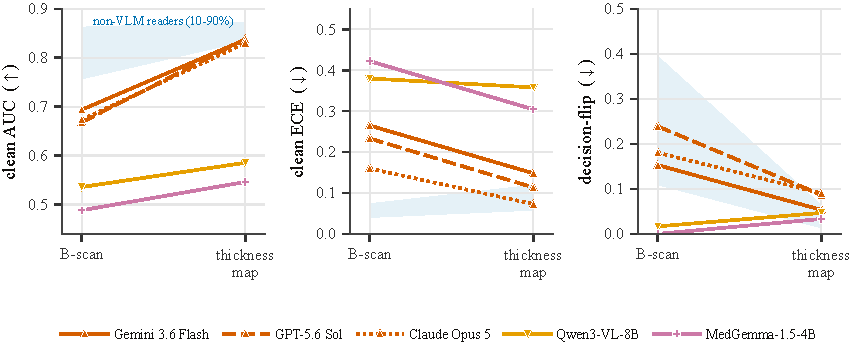
\includegraphics[width=0.72\linewidth]{figures/figA4_grounding.pdf}
  \caption{\textbf{The per-VLM thickness-map improvement, in three metrics.} Per-VLM change from the raw B-scan to the color
  thickness-map render (few-shot); the three frontier VLMs share the vermilion triangle and are distinguished by
  line style. The stronger frontier VLMs rise into the per-axis non-VLM reader band (10--90th percentile of the FM
  and CNN readers) on clean AUC and descend toward it on ECE and decision-flip together. The small open
  (Qwen3-VL-8B) and specialist (MedGemma-1.5-4B) models do not recover.}
  \label{fig:grounding}
\end{figure}

\section{Subgroup robustness}
\label{app:subgroups}
We ask whether the scanner-induced instability falls unevenly across disease severity or demographics, recomputing
decision-flip per subgroup for every configuration on the seed-0 test split
(\texttt{scripts/analyze\_subgroups.py}). Fig.~\ref{fig:subgroups} aggregates this by the four
capable reader classes (class mean and across-model spread; the near-chance open/specialist VLMs are near-constant and
omitted from the figure), and Tables~\ref{tab:sev}--\ref{tab:demo} give the per-reader point estimates for all
configurations. Decision-flip stays broadly comparable across subgroups. No severity grade or demographic group
shows a consistently elevated flip once the wide eye-level bootstrap CIs are accounted for. The one clear pattern is the B-scan over-referral of \S\ref{sec:findings}: for the appearance-keyed
readers the \emph{healthy} eyes flip most (MIRAGE\,$\cdot$\,LP \num{0.62} vs.\ \num{0.28} moderate/advanced; RETFound\,$\cdot$\,LP
\num{0.47} vs.\ \num{0.09}; SmallCNN \num{0.35} vs.\ \num{0.15}), i.e.\ the false-referral load concentrates in the
screening-relevant non-glaucoma population. Sensitivity change ($\Delta$sens) is likewise small and CI-overlapping
across the glaucoma severity subgroups. \emph{Caveats}: the GLEAM severity subgroups are small ($n\approx 57$--$184$ per
grade, so 95\% CIs span $\approx\pm0.08$--$0.13$); \textbf{image quality is not recorded in either dataset} and GLEAM
carries no demographics, so those subgroup axes cannot be tested and are left to future work.

\begin{figure}[tbp]
  \centering
  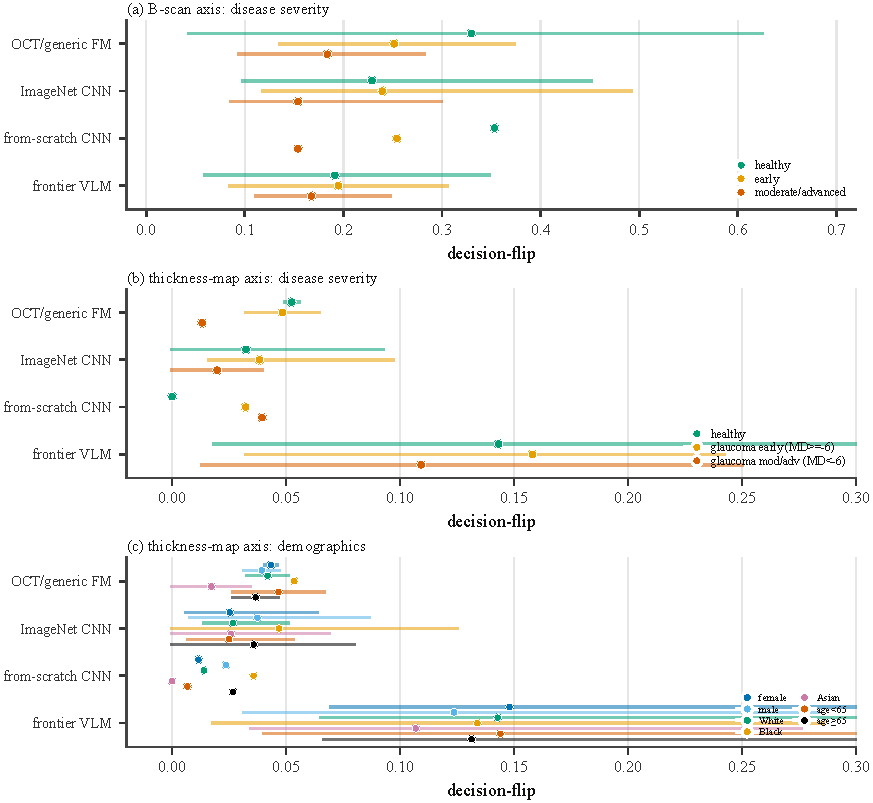
\includegraphics[width=0.86\linewidth]{figures/figA5_subgroups.pdf}
  \caption{\textbf{Decision-flip by subgroup, aggregated by reader class} (the four capable Fig.~\ref{fig:stability}
  classes; the near-constant open/specialist VLMs are omitted here but listed in Tables~\ref{tab:sev}--\ref{tab:demo}).
  Markers are the class mean across its models; bars span the min--max across those models. \textbf{(a)}~B-scan
  disease severity: for the appearance-keyed classes (OCT/generic FM, ImageNet CNN, from-scratch CNN) the healthy-eye
  flip is highest (over-referral on the screening population; the wide bars are within-class model spread, e.g.\ robust
  DINOv2\,$\cdot$\,FT vs.\ unstable MIRAGE\,$\cdot$\,LP), whereas the frontier VLMs are flat. \textbf{(b)}~Thickness-map
  severity and \textbf{(c)}~map demographics: flip stays low and the subgroups cluster for every class, with no group
  consistently elevated. The flip scale differs between (a) and (b,c).}
  \label{fig:subgroups}
\end{figure}

% auto-generated by scripts/build_paper_tables.py — do not edit by hand
\begin{table}[tbp]
  \centering
  \caption{\textbf{Decision-flip by disease severity}, both axes, all configurations (point estimates; the per-reader eye-level bootstrap 95\% CIs are wide and overlapping across grades, and the class-aggregated means and model spread are in Fig.~\ref{fig:subgroups}a,b). Severity: B-scan from the GLEAM 4-class label (healthy / early / moderate-advanced); map from Harvard-GDP mean deviation (healthy / MD$\ge-6$ / MD$<-6$). ``--'' = reader not run on that axis.}
  \label{tab:sev}
  \small
  \renewcommand{\arraystretch}{0.9}
  \setlength{\tabcolsep}{5pt}
  \begin{tabular}{lcccccc}
    \toprule
    & \multicolumn{3}{c}{B-scan axis} & \multicolumn{3}{c}{Thickness-map axis} \\
    \cmidrule(lr){2-4}\cmidrule(lr){5-7}
    Reader & healthy & early & mod/adv & healthy & early & mod/adv \\
    \midrule
    DINOv2\,$\cdot$\,FT & 0.04 & 0.14 & 0.13 & 0.05 & 0.03 & 0.01 \\
    DINOv2\,$\cdot$\,LP & 0.18 & 0.14 & 0.24 & 0.06 & 0.06 & 0.01 \\
    MIRAGE\,$\cdot$\,FT & 0.51 & 0.34 & 0.25 & -- & -- & -- \\
    MIRAGE\,$\cdot$\,LP & 0.62 & 0.37 & 0.28 & -- & -- & -- \\
    RETFound\,$\cdot$\,FT & 0.15 & 0.17 & 0.11 & -- & -- & -- \\
    RETFound\,$\cdot$\,LP & 0.47 & 0.36 & 0.09 & -- & -- & -- \\
    ConvNeXt-B\,$\cdot$\,FT & 0.16 & 0.15 & 0.09 & 0.00 & 0.02 & 0.03 \\
    ConvNeXt-B\,$\cdot$\,LP & 0.10 & 0.15 & 0.09 & 0.02 & 0.02 & 0.00 \\
    ConvNeXt-L\,$\cdot$\,FT & 0.18 & 0.19 & 0.09 & 0.01 & 0.03 & 0.03 \\
    ConvNeXt-L\,$\cdot$\,LP & 0.17 & 0.19 & 0.15 & 0.04 & 0.06 & 0.01 \\
    ConvNeXt-T\,$\cdot$\,FT & 0.12 & 0.12 & 0.09 & 0.02 & 0.02 & 0.00 \\
    ConvNeXt-T\,$\cdot$\,LP & 0.41 & 0.37 & 0.16 & 0.01 & 0.03 & 0.03 \\
    ResNet-50\,$\cdot$\,FT & 0.45 & 0.49 & 0.26 & 0.09 & 0.03 & 0.03 \\
    ResNet-50\,$\cdot$\,LP & 0.23 & 0.25 & 0.30 & 0.06 & 0.10 & 0.04 \\
    SmallCNN (98k) & 0.35 & 0.25 & 0.15 & 0.00 & 0.03 & 0.04 \\
    Claude Opus~5\,\textit{fs} & 0.23 & 0.17 & 0.11 & 0.10 & 0.11 & 0.04 \\
    Claude Opus~5\,\textit{zs} & 0.35 & 0.24 & 0.16 & 0.03 & 0.18 & 0.08 \\
    GPT-5.6 Sol\,\textit{fs} & 0.21 & 0.31 & 0.25 & 0.10 & 0.10 & 0.04 \\
    GPT-5.6 Sol\,\textit{zs} & 0.06 & 0.08 & 0.11 & 0.02 & 0.16 & 0.18 \\
    Gemini 2.5 Flash\,\textit{fs} & 0.20 & 0.29 & 0.19 & 0.30 & 0.23 & 0.09 \\
    Gemini 2.5 Flash\,\textit{zs} & 0.10 & 0.12 & 0.11 & 0.37 & 0.19 & 0.25 \\
    Gemini 2.5 Pro\,\textit{fs} & 0.27 & 0.19 & 0.21 & 0.17 & 0.18 & 0.09 \\
    Gemini 2.5 Pro\,\textit{zs} & 0.12 & 0.17 & 0.14 & 0.24 & 0.24 & 0.18 \\
    Gemini 3.6 Flash\,\textit{fs} & 0.14 & 0.20 & 0.15 & 0.08 & 0.03 & 0.01 \\
    Gemini 3.6 Flash\,\textit{zs} & 0.23 & 0.19 & 0.25 & 0.02 & 0.16 & 0.12 \\
    Qwen3-VL-8B\,\textit{fs} & 0.02 & 0.02 & 0.01 & 0.07 & 0.02 & 0.01 \\
    Qwen3-VL-8B\,\textit{zs} & 0.21 & 0.17 & 0.15 & 0.01 & 0.00 & 0.00 \\
    MedGemma-1.5-4B\,\textit{fs} & 0.00 & 0.00 & 0.00 & 0.02 & 0.08 & 0.01 \\
    MedGemma-1.5-4B\,\textit{zs} & 0.00 & 0.00 & 0.00 & 0.02 & 0.03 & 0.00 \\
    \bottomrule
  \end{tabular}
\end{table}

\begin{table}[tbp]
  \centering
  \caption{\textbf{Decision-flip by demographics} (thickness-map axis, Harvard-GDP; all configurations, point estimates, wide overlapping CIs; class-aggregated view in Fig.~\ref{fig:subgroups}c). No group is consistently elevated. GLEAM (B-scan) carries no demographics.}
  \label{tab:demo}
  \small
  \renewcommand{\arraystretch}{0.9}
  \setlength{\tabcolsep}{5pt}
  \begin{tabular}{lccccccc}
    \toprule
    & \multicolumn{2}{c}{gender} & \multicolumn{3}{c}{race} & \multicolumn{2}{c}{age} \\
    \cmidrule(lr){2-3}\cmidrule(lr){4-6}\cmidrule(lr){7-8}
    Reader & F & M & White & Black & Asian & $<$65 & $\ge$65 \\
    \midrule
    DINOv2\,$\cdot$\,FT & 0.04 & 0.03 & 0.03 & 0.05 & 0.03 & 0.03 & 0.05 \\
    DINOv2\,$\cdot$\,LP & 0.05 & 0.05 & 0.05 & 0.05 & 0.00 & 0.07 & 0.03 \\
    ConvNeXt-B\,$\cdot$\,FT & 0.01 & 0.01 & 0.01 & 0.00 & 0.00 & 0.02 & 0.00 \\
    ConvNeXt-B\,$\cdot$\,LP & 0.01 & 0.02 & 0.02 & 0.00 & 0.00 & 0.01 & 0.01 \\
    ConvNeXt-L\,$\cdot$\,FT & 0.01 & 0.02 & 0.01 & 0.04 & 0.00 & 0.01 & 0.03 \\
    ConvNeXt-L\,$\cdot$\,LP & 0.03 & 0.05 & 0.04 & 0.04 & 0.07 & 0.03 & 0.05 \\
    ConvNeXt-T\,$\cdot$\,FT & 0.01 & 0.02 & 0.01 & 0.04 & 0.00 & 0.01 & 0.02 \\
    ConvNeXt-T\,$\cdot$\,LP & 0.02 & 0.02 & 0.02 & 0.02 & 0.03 & 0.01 & 0.03 \\
    ResNet-50\,$\cdot$\,FT & 0.06 & 0.06 & 0.05 & 0.12 & 0.07 & 0.05 & 0.08 \\
    ResNet-50\,$\cdot$\,LP & 0.05 & 0.09 & 0.05 & 0.12 & 0.03 & 0.05 & 0.07 \\
    SmallCNN (98k) & 0.01 & 0.02 & 0.01 & 0.04 & 0.00 & 0.01 & 0.03 \\
    Claude Opus~5\,\textit{fs} & 0.11 & 0.06 & 0.08 & 0.11 & 0.10 & 0.09 & 0.09 \\
    Claude Opus~5\,\textit{zs} & 0.08 & 0.07 & 0.07 & 0.11 & 0.03 & 0.08 & 0.07 \\
    GPT-5.6 Sol\,\textit{fs} & 0.11 & 0.06 & 0.08 & 0.11 & 0.07 & 0.10 & 0.07 \\
    GPT-5.6 Sol\,\textit{zs} & 0.09 & 0.09 & 0.08 & 0.14 & 0.03 & 0.09 & 0.09 \\
    Gemini 2.5 Flash\,\textit{fs} & 0.25 & 0.20 & 0.22 & 0.23 & 0.28 & 0.24 & 0.22 \\
    Gemini 2.5 Flash\,\textit{zs} & 0.32 & 0.28 & 0.33 & 0.29 & 0.17 & 0.30 & 0.31 \\
    Gemini 2.5 Pro\,\textit{fs} & 0.16 & 0.14 & 0.17 & 0.12 & 0.07 & 0.19 & 0.11 \\
    Gemini 2.5 Pro\,\textit{zs} & 0.24 & 0.21 & 0.26 & 0.14 & 0.17 & 0.25 & 0.20 \\
    Gemini 3.6 Flash\,\textit{fs} & 0.07 & 0.03 & 0.07 & 0.02 & 0.03 & 0.04 & 0.07 \\
    Gemini 3.6 Flash\,\textit{zs} & 0.07 & 0.08 & 0.07 & 0.07 & 0.10 & 0.07 & 0.08 \\
    Qwen3-VL-8B\,\textit{fs} & 0.06 & 0.03 & 0.05 & 0.05 & 0.03 & 0.07 & 0.03 \\
    Qwen3-VL-8B\,\textit{zs} & 0.00 & 0.01 & 0.00 & 0.00 & 0.00 & 0.01 & 0.00 \\
    MedGemma-1.5-4B\,\textit{fs} & 0.03 & 0.04 & 0.03 & 0.05 & 0.03 & 0.03 & 0.03 \\
    MedGemma-1.5-4B\,\textit{zs} & 0.03 & 0.01 & 0.01 & 0.00 & 0.10 & 0.03 & 0.01 \\
    \bottomrule
  \end{tabular}
\end{table}


\section{Full per-axis tables}
\label{app:fulltables}
% auto-generated by scripts/build_paper_tables.py — do not edit by hand
\begin{table}[h]
  \centering
  \caption{\textbf{Full B-scan (appearance) axis, all 29 configurations}. Spectralis\,$\rightarrow$\,Topcon speckle shift ($n{=}360$ eyes). spec@shift = realized specificity under the shift at the 90\%-specificity operating point (a low value signals decision collapse); ECE, aECE and Brier have no bootstrap CI in the released summaries. ECE is the positive-class calibration error (10 equal-width bins); aECE is the adaptive (equal-mass) ECE and Brier is the Brier score, a strictly proper score with no binning, so together they show the calibration reads are not a fixed-bin artifact. NCE $=$ net calibration error, a signed calibration error \citep{groot2024overconfidence} (mean predicted-class confidence minus accuracy; $+$ $=$ overconfident). All calibration reads are on the clean eyes.}
  \small
  \setlength{\tabcolsep}{3pt}
  \resizebox{\linewidth}{!}{%
  \begin{tabular}{llccccccccc}
    \toprule
    Reader & Class & AUC \ci{95\%}{CI} & Flip \ci{95\%}{CI} & $\Delta$sens \ci{95\%}{CI} & spec@shift & ECE & aECE & Brier & NCE & $\Delta$AUC \\
    \midrule
    DINOv2\,$\cdot$\,FT & FM & 0.876 \ci{0.84}{0.91} & 0.086 \ci{0.06}{0.12} & +0.080 \ci{0.03}{0.13} & 0.92 & 0.052 & 0.073 & 0.145 & -0.003 & +0.011 \\
    RETFound\,$\cdot$\,FT & FM & 0.847 \ci{0.80}{0.89} & 0.142 \ci{0.11}{0.18} & -0.091 \ci{-0.14}{-0.04} & 0.81 & 0.072 & 0.080 & 0.158 & +0.067 & -0.007 \\
    RETFound\,$\cdot$\,LP & FM & 0.845 \ci{0.80}{0.88} & 0.328 \ci{0.28}{0.38} & -0.227 \ci{-0.29}{-0.16} & 0.52 & 0.040 & 0.035 & 0.160 & -0.001 & +0.061 \\
    DINOv2\,$\cdot$\,LP & FM & 0.842 \ci{0.80}{0.88} & 0.194 \ci{0.16}{0.24} & +0.165 \ci{0.10}{0.23} & 0.92 & 0.047 & 0.039 & 0.162 & +0.034 & +0.059 \\
    MIRAGE\,$\cdot$\,FT & FM & 0.736 \ci{0.68}{0.78} & 0.394 \ci{0.34}{0.44} & -0.386 \ci{-0.46}{-0.32} & 0.61 & 0.121 & 0.119 & 0.220 & +0.097 & -0.002 \\
    MIRAGE\,$\cdot$\,LP & FM & 0.701 \ci{0.65}{0.76} & 0.472 \ci{0.42}{0.52} & -0.722 \ci{-0.79}{-0.65} & 0.07 & 0.041 & 0.067 & 0.221 & -0.021 & +0.044 \\
    ConvNeXt-T\,$\cdot$\,FT & ImageNet CNN & 0.869 \ci{0.83}{0.90} & 0.111 \ci{0.08}{0.14} & -0.097 \ci{-0.14}{-0.06} & 0.68 & 0.067 & 0.070 & 0.147 & -0.003 & +0.026 \\
    ConvNeXt-B\,$\cdot$\,FT & ImageNet CNN & 0.854 \ci{0.81}{0.89} & 0.136 \ci{0.10}{0.17} & -0.051 \ci{-0.10}{0.01} & 0.74 & 0.049 & 0.067 & 0.155 & -0.019 & +0.050 \\
    ConvNeXt-L\,$\cdot$\,FT & ImageNet CNN & 0.836 \ci{0.79}{0.87} & 0.153 \ci{0.12}{0.19} & -0.068 \ci{-0.12}{-0.02} & 0.76 & 0.066 & 0.067 & 0.164 & +0.051 & +0.045 \\
    ResNet-50\,$\cdot$\,FT & ImageNet CNN & 0.833 \ci{0.78}{0.87} & 0.394 \ci{0.34}{0.44} & -0.307 \ci{-0.37}{-0.24} & 0.55 & 0.068 & 0.078 & 0.169 & +0.035 & +0.006 \\
    ConvNeXt-B\,$\cdot$\,LP & ImageNet CNN & 0.826 \ci{0.78}{0.87} & 0.108 \ci{0.07}{0.14} & +0.068 \ci{0.02}{0.13} & 0.91 & 0.070 & 0.055 & 0.170 & +0.029 & +0.038 \\
    ConvNeXt-T\,$\cdot$\,LP & ImageNet CNN & 0.826 \ci{0.78}{0.87} & 0.325 \ci{0.28}{0.38} & -0.199 \ci{-0.26}{-0.14} & 0.60 & 0.036 & 0.051 & 0.169 & +0.031 & +0.038 \\
    ConvNeXt-L\,$\cdot$\,LP & ImageNet CNN & 0.825 \ci{0.78}{0.86} & 0.167 \ci{0.13}{0.21} & +0.028 \ci{-0.03}{0.09} & 0.83 & 0.062 & 0.058 & 0.168 & +0.014 & +0.048 \\
    ResNet-50\,$\cdot$\,LP & ImageNet CNN & 0.825 \ci{0.78}{0.86} & 0.258 \ci{0.22}{0.30} & +0.136 \ci{0.06}{0.21} & 0.89 & 0.075 & 0.076 & 0.174 & +0.027 & +0.080 \\
    SmallCNN (98k) & scratch CNN & 0.788 \ci{0.74}{0.83} & 0.272 \ci{0.23}{0.32} & -0.324 \ci{-0.40}{-0.25} & 0.65 & 0.042 & 0.063 & 0.189 & -0.039 & +0.017 \\
    Gemini 3.6 Flash\,\textit{fs} & frontier VLM & 0.694 \ci{0.64}{0.74} & 0.153 \ci{0.12}{0.19} & +0.006 \ci{-0.03}{0.04} & 0.90 & 0.265 & 0.260 & 0.292 & +0.258 & -0.001 \\
    Claude Opus~5\,\textit{fs} & frontier VLM & 0.673 \ci{0.62}{0.73} & 0.181 \ci{0.14}{0.22} & +0.045 \ci{0.00}{0.09} & 0.97 & 0.160 & 0.159 & 0.253 & +0.132 & +0.030 \\
    GPT-5.6 Sol\,\textit{fs} & frontier VLM & 0.668 \ci{0.61}{0.73} & 0.239 \ci{0.19}{0.28} & +0.108 \ci{0.05}{0.17} & 0.92 & 0.233 & 0.218 & 0.283 & +0.228 & -0.012 \\
    Gemini 2.5 Pro\,\textit{fs} & frontier VLM & 0.635 \ci{0.58}{0.69} & 0.239 \ci{0.20}{0.28} & -0.017 \ci{-0.06}{0.02} & 0.99 & 0.324 & 0.313 & 0.338 & +0.322 & -0.004 \\
    GPT-5.6 Sol\,\textit{zs} & frontier VLM & 0.631 \ci{0.58}{0.69} & 0.081 \ci{0.06}{0.11} & +0.045 \ci{-0.02}{0.11} & 0.92 & 0.307 & 0.297 & 0.337 & +0.304 & -0.004 \\
    Gemini 2.5 Flash\,\textit{fs} & frontier VLM & 0.622 \ci{0.57}{0.68} & 0.211 \ci{0.17}{0.25} & +0.040 \ci{-0.01}{0.09} & 0.95 & 0.297 & 0.279 & 0.325 & +0.295 & +0.013 \\
    Claude Opus~5\,\textit{zs} & frontier VLM & 0.607 \ci{0.55}{0.66} & 0.269 \ci{0.22}{0.31} & -0.034 \ci{-0.09}{0.02} & 0.97 & 0.113 & 0.090 & 0.250 & +0.076 & +0.010 \\
    Gemini 3.6 Flash\,\textit{zs} & frontier VLM & 0.596 \ci{0.54}{0.65} & 0.228 \ci{0.19}{0.27} & -0.011 \ci{-0.08}{0.05} & 0.89 & 0.356 & 0.308 & 0.368 & +0.349 & +0.032 \\
    Gemini 2.5 Flash\,\textit{zs} & frontier VLM & 0.571 \ci{0.52}{0.62} & 0.108 \ci{0.08}{0.14} & +0.023 \ci{-0.03}{0.08} & 0.91 & 0.390 & 0.372 & 0.399 & +0.379 & +0.053 \\
    Gemini 2.5 Pro\,\textit{zs} & frontier VLM & 0.515 \ci{0.47}{0.56} & 0.133 \ci{0.10}{0.17} & +0.023 \ci{-0.04}{0.09} & 0.92 & 0.422 & 0.407 & 0.427 & +0.420 & -0.029 \\
    Qwen3-VL-8B\,\textit{fs} & open VLM & 0.536 \ci{0.49}{0.58} & 0.017 \ci{0.01}{0.03} & +0.000 \ci{0.00}{0.00} & 1.00 & 0.380 & 0.369 & 0.393 & +0.380 & +0.000 \\
    Qwen3-VL-8B\,\textit{zs} & open VLM & 0.462 \ci{0.42}{0.50} & 0.186 \ci{0.15}{0.23} & +0.000 \ci{0.00}{0.00} & 1.00 & 0.510 & 0.487 & 0.510 & +0.510 & +0.038 \\
    MedGemma-1.5-4B\,\textit{zs} & specialist VLM & 0.539 \ci{0.49}{0.58} & 0.000 \ci{0.00}{0.00} & +0.023 \ci{-0.01}{0.05} & 0.99 & 0.464 & 0.465 & 0.463 & +0.465 & -0.015 \\
    MedGemma-1.5-4B\,\textit{fs} & specialist VLM & 0.488 \ci{0.43}{0.54} & 0.000 \ci{0.00}{0.00} & +0.034 \ci{0.00}{0.07} & 0.98 & 0.422 & 0.422 & 0.430 & +0.422 & -0.036 \\
    \bottomrule
  \end{tabular}}
\end{table}

\begin{table}[h]
  \centering
  \caption{\textbf{Full thickness-map (color-map) axis, all 25 configurations}. Cirrus\,$\rightarrow$\,Spectralis offset; OCT-specific B-scan FMs are not run on map renders ($n{=}300$ eyes). spec@shift = realized specificity under the shift at the 90\%-specificity operating point (a low value signals decision collapse); ECE, aECE and Brier have no bootstrap CI in the released summaries. ECE is the positive-class calibration error (10 equal-width bins); aECE is the adaptive (equal-mass) ECE and Brier is the Brier score, a strictly proper score with no binning, so together they show the calibration reads are not a fixed-bin artifact. NCE $=$ net calibration error, a signed calibration error \citep{groot2024overconfidence} (mean predicted-class confidence minus accuracy; $+$ $=$ overconfident). All calibration reads are on the clean eyes.}
  \small
  \setlength{\tabcolsep}{3pt}
  \resizebox{\linewidth}{!}{%
  \begin{tabular}{llccccccccc}
    \toprule
    Reader & Class & AUC \ci{95\%}{CI} & Flip \ci{95\%}{CI} & $\Delta$sens \ci{95\%}{CI} & spec@shift & ECE & aECE & Brier & NCE & $\Delta$AUC \\
    \midrule
    DINOv2\,$\cdot$\,FT & FM & 0.876 \ci{0.83}{0.91} & 0.037 \ci{0.02}{0.06} & +0.014 \ci{-0.01}{0.04} & 0.93 & 0.090 & 0.089 & 0.136 & -0.018 & +0.004 \\
    DINOv2\,$\cdot$\,LP & FM & 0.849 \ci{0.80}{0.89} & 0.047 \ci{0.02}{0.07} & +0.029 \ci{-0.01}{0.07} & 0.90 & 0.078 & 0.062 & 0.153 & +0.035 & -0.001 \\
    ConvNeXt-L\,$\cdot$\,FT & ImageNet CNN & 0.872 \ci{0.83}{0.91} & 0.017 \ci{0.00}{0.03} & +0.007 \ci{-0.02}{0.03} & 0.91 & 0.067 & 0.074 & 0.137 & -0.040 & +0.001 \\
    ResNet-50\,$\cdot$\,FT & ImageNet CNN & 0.865 \ci{0.82}{0.91} & 0.063 \ci{0.04}{0.09} & +0.007 \ci{-0.02}{0.03} & 0.96 & 0.135 & 0.130 & 0.152 & -0.085 & -0.005 \\
    ConvNeXt-T\,$\cdot$\,FT & ImageNet CNN & 0.862 \ci{0.82}{0.91} & 0.017 \ci{0.00}{0.03} & +0.000 \ci{-0.03}{0.03} & 0.91 & 0.095 & 0.098 & 0.141 & -0.037 & -0.000 \\
    ConvNeXt-B\,$\cdot$\,FT & ImageNet CNN & 0.859 \ci{0.81}{0.90} & 0.010 \ci{0.00}{0.02} & +0.000 \ci{0.00}{0.00} & 0.91 & 0.112 & 0.169 & 0.170 & +0.011 & -0.001 \\
    ConvNeXt-B\,$\cdot$\,LP & ImageNet CNN & 0.843 \ci{0.79}{0.89} & 0.013 \ci{0.00}{0.03} & -0.014 \ci{-0.04}{0.01} & 0.90 & 0.057 & 0.065 & 0.151 & +0.021 & -0.001 \\
    ConvNeXt-T\,$\cdot$\,LP & ImageNet CNN & 0.836 \ci{0.79}{0.88} & 0.020 \ci{0.01}{0.04} & +0.058 \ci{0.02}{0.10} & 0.93 & 0.058 & 0.066 & 0.155 & +0.001 & -0.001 \\
    ConvNeXt-L\,$\cdot$\,LP & ImageNet CNN & 0.834 \ci{0.78}{0.88} & 0.040 \ci{0.02}{0.06} & -0.007 \ci{-0.03}{0.02} & 0.89 & 0.081 & 0.054 & 0.156 & +0.059 & -0.008 \\
    ResNet-50\,$\cdot$\,LP & ImageNet CNN & 0.831 \ci{0.78}{0.88} & 0.063 \ci{0.04}{0.09} & -0.007 \ci{-0.04}{0.03} & 0.88 & 0.058 & 0.067 & 0.163 & +0.029 & +0.014 \\
    SmallCNN (98k) & scratch CNN & 0.847 \ci{0.80}{0.89} & 0.017 \ci{0.00}{0.03} & +0.000 \ci{-0.04}{0.04} & 0.94 & 0.119 & 0.139 & 0.169 & +0.033 & -0.006 \\
    Claude Opus~5\,\textit{zs} & frontier VLM & 0.850 \ci{0.81}{0.89} & 0.073 \ci{0.05}{0.10} & +0.058 \ci{0.00}{0.12} & 0.93 & 0.106 & 0.113 & 0.167 & -0.011 & +0.023 \\
    GPT-5.6 Sol\,\textit{fs} & frontier VLM & 0.838 \ci{0.79}{0.88} & 0.087 \ci{0.06}{0.12} & +0.022 \ci{-0.03}{0.07} & 0.93 & 0.113 & 0.110 & 0.170 & +0.110 & -0.005 \\
    Gemini 3.6 Flash\,\textit{fs} & frontier VLM & 0.837 \ci{0.79}{0.88} & 0.053 \ci{0.03}{0.08} & +0.058 \ci{0.02}{0.09} & 0.93 & 0.148 & 0.140 & 0.175 & +0.134 & +0.016 \\
    Claude Opus~5\,\textit{fs} & frontier VLM & 0.830 \ci{0.78}{0.88} & 0.090 \ci{0.06}{0.12} & +0.029 \ci{-0.01}{0.07} & 0.93 & 0.073 & 0.074 & 0.161 & +0.014 & -0.002 \\
    Gemini 2.5 Pro\,\textit{fs} & frontier VLM & 0.807 \ci{0.76}{0.86} & 0.150 \ci{0.11}{0.19} & -0.051 \ci{-0.12}{0.01} & 0.96 & 0.150 & 0.153 & 0.189 & +0.150 & -0.007 \\
    Gemini 3.6 Flash\,\textit{zs} & frontier VLM & 0.797 \ci{0.75}{0.85} & 0.073 \ci{0.05}{0.10} & +0.043 \ci{-0.01}{0.11} & 0.94 & 0.230 & 0.226 & 0.239 & +0.201 & -0.006 \\
    Gemini 2.5 Flash\,\textit{fs} & frontier VLM & 0.775 \ci{0.72}{0.82} & 0.230 \ci{0.19}{0.28} & -0.029 \ci{-0.11}{0.04} & 0.94 & 0.173 & 0.147 & 0.218 & +0.169 & -0.001 \\
    GPT-5.6 Sol\,\textit{zs} & frontier VLM & 0.772 \ci{0.72}{0.82} & 0.090 \ci{0.06}{0.12} & -0.014 \ci{-0.09}{0.06} & 0.90 & 0.233 & 0.227 & 0.241 & +0.170 & -0.026 \\
    Gemini 2.5 Pro\,\textit{zs} & frontier VLM & 0.713 \ci{0.66}{0.77} & 0.227 \ci{0.18}{0.28} & -0.007 \ci{-0.09}{0.08} & 0.98 & 0.268 & 0.261 & 0.282 & +0.266 & +0.004 \\
    Gemini 2.5 Flash\,\textit{zs} & frontier VLM & 0.644 \ci{0.58}{0.71} & 0.303 \ci{0.26}{0.35} & +0.036 \ci{-0.03}{0.10} & 1.00 & 0.229 & 0.221 & 0.287 & +0.211 & -0.026 \\
    Qwen3-VL-8B\,\textit{fs} & open VLM & 0.585 \ci{0.55}{0.62} & 0.047 \ci{0.02}{0.07} & +0.000 \ci{-0.04}{0.04} & 0.94 & 0.358 & 0.345 & 0.369 & +0.358 & +0.018 \\
    Qwen3-VL-8B\,\textit{zs} & open VLM & 0.500 \ci{0.50}{0.50} & 0.003 \ci{0.00}{0.01} & +0.000 \ci{0.00}{0.00} & 1.00 & 0.490 & 0.490 & 0.489 & +0.490 & -0.003 \\
    MedGemma-1.5-4B\,\textit{fs} & specialist VLM & 0.546 \ci{0.48}{0.61} & 0.033 \ci{0.02}{0.06} & +0.000 \ci{-0.04}{0.04} & 0.92 & 0.304 & 0.291 & 0.341 & +0.299 & +0.025 \\
    MedGemma-1.5-4B\,\textit{zs} & specialist VLM & 0.411 \ci{0.35}{0.47} & 0.020 \ci{0.01}{0.04} & -0.014 \ci{-0.04}{0.00} & 0.95 & 0.384 & 0.364 & 0.406 & +0.379 & +0.018 \\
    \bottomrule
  \end{tabular}}
\end{table}


\section{Reproducibility and broader impact}
\label{app:repro}

\paragraph{Reproducibility.} We release the full pipeline, the verbatim prompts (\S\ref{app:prompts}), the per-configuration
model IDs and inference settings (Table~\ref{tab:models}), and all seeds. Splits are eye-level and seed-fixed;
encoder probes are fit on the seed-0 split; VLM elicitation is greedy (single sample). Because
frontier API models drift, we pin each model ID and API date and archive the raw per-eye model responses, so every
table and figure reproduces exactly from the released code and responses; re-querying a live API may differ as the
served model changes. On acceptance we release, under the MIT license, the exact synthetic-shift transforms (the
B-scan appearance transform and the thickness-map scanner-offset, with every parameter and per-eye seed) together
with the committed per-eye outputs, so a new model can be scored directly against the calibrated shift; the
datasets remain under their own access terms (GLEAM; Harvard-GDP CC BY-NC-ND 4.0; GOALS; RETOUCH).

\paragraph{Broader impact.} The deployment-relevant finding is a safety one: a reader can preserve AUC under
a scanner change while its diagnostic decisions flip, so a naive AUC-only validation can
license an unsafe glaucoma-diagnosis reader. We advocate decision-level, calibration-aware, shift-aware evaluation
before deployment, and release the benchmark as a reusable check. The study uses de-identified public research
datasets; no new patient data were collected.


% flush all deferred appendix floats (tables/figures) so the checklist starts after them
\clearpage
\section*{NeurIPS Paper Checklist}



\begin{enumerate}

\item {\bf Claims}
    \item[] Question: Do the main claims made in the abstract and introduction accurately reflect the paper's contributions and scope?
    \item[] Answer: \answerYes{}
    \item[] Justification: The abstract's four numbered findings map to F1--F4 (\S\ref{sec:findings}) and are each supported by eye-level bootstrap confidence intervals; the scope (two axes, never cross-ranked) is stated explicitly.
    \item[] Guidelines:
    \begin{itemize}
        \item The answer \answerNA{} means that the abstract and introduction do not include the claims made in the paper.
        \item The abstract and/or introduction should clearly state the claims made, including the contributions made in the paper and important assumptions and limitations. A \answerNo{} or \answerNA{} answer to this question will not be perceived well by the reviewers. 
        \item The claims made should match theoretical and experimental results, and reflect how much the results can be expected to generalize to other settings. 
        \item It is fine to include aspirational goals as motivation as long as it is clear that these goals are not attained by the paper. 
    \end{itemize}

\item {\bf Limitations}
    \item[] Question: Does the paper discuss the limitations of the work performed by the authors?
    \item[] Answer: \answerYes{}
    \item[] Justification: The Limitations paragraph (\S\ref{sec:discussion}) discusses the synthetic same-eye shift, the conservative single greedy verbalized-probability elicitation, the cross-dataset F2 comparison, the underpowered subgroups and missing image-quality field, and the cross-sectional two-axis scope.
    \item[] Guidelines:
    \begin{itemize}
        \item The answer \answerNA{} means that the paper has no limitation while the answer \answerNo{} means that the paper has limitations, but those are not discussed in the paper. 
        \item The authors are encouraged to create a separate ``Limitations'' section in their paper.
        \item The paper should point out any strong assumptions and how robust the results are to violations of these assumptions (e.g., independence assumptions, noiseless settings, model well-specification, asymptotic approximations only holding locally). The authors should reflect on how these assumptions might be violated in practice and what the implications would be.
        \item The authors should reflect on the scope of the claims made, e.g., if the approach was only tested on a few datasets or with a few runs. In general, empirical results often depend on implicit assumptions, which should be articulated.
        \item The authors should reflect on the factors that influence the performance of the approach. For example, a facial recognition algorithm may perform poorly when image resolution is low or images are taken in low lighting. Or a speech-to-text system might not be used reliably to provide closed captions for online lectures because it fails to handle technical jargon.
        \item The authors should discuss the computational efficiency of the proposed algorithms and how they scale with dataset size.
        \item If applicable, the authors should discuss possible limitations of their approach to address problems of privacy and fairness.
        \item While the authors might fear that complete honesty about limitations might be used by reviewers as grounds for rejection, a worse outcome might be that reviewers discover limitations that aren't acknowledged in the paper. The authors should use their best judgment and recognize that individual actions in favor of transparency play an important role in developing norms that preserve the integrity of the community. Reviewers will be specifically instructed to not penalize honesty concerning limitations.
    \end{itemize}

\item {\bf Theory assumptions and proofs}
    \item[] Question: For each theoretical result, does the paper provide the full set of assumptions and a complete (and correct) proof?
    \item[] Answer: \answerNA{}
    \item[] Justification: The paper contains no theoretical results.
    \item[] Guidelines:
    \begin{itemize}
        \item The answer \answerNA{} means that the paper does not include theoretical results. 
        \item All the theorems, formulas, and proofs in the paper should be numbered and cross-referenced.
        \item All assumptions should be clearly stated or referenced in the statement of any theorems.
        \item The proofs can either appear in the main paper or the supplemental material, but if they appear in the supplemental material, the authors are encouraged to provide a short proof sketch to provide intuition. 
        \item Inversely, any informal proof provided in the core of the paper should be complemented by formal proofs provided in appendix or supplemental material.
        \item Theorems and Lemmas that the proof relies upon should be properly referenced. 
    \end{itemize}

    \item {\bf Experimental result reproducibility}
    \item[] Question: Does the paper fully disclose all the information needed to reproduce the main experimental results of the paper to the extent that it affects the main claims and/or conclusions of the paper (regardless of whether the code and data are provided or not)?
    \item[] Answer: \answerYes{}
    \item[] Justification: We disclose the full pipeline, the verbatim prompts (App.~\ref{app:prompts}), the per-configuration model identifiers and inference settings (Table~\ref{tab:models}), and all seeds; FM/CNN probabilities reproduce from cached features with the frozen probe, and the raw per-eye VLM responses are archived (App.~\ref{app:repro}).
    \item[] Guidelines:
    \begin{itemize}
        \item The answer \answerNA{} means that the paper does not include experiments.
        \item If the paper includes experiments, a \answerNo{} answer to this question will not be perceived well by the reviewers: Making the paper reproducible is important, regardless of whether the code and data are provided or not.
        \item If the contribution is a dataset and\slash or model, the authors should describe the steps taken to make their results reproducible or verifiable. 
        \item Depending on the contribution, reproducibility can be accomplished in various ways. For example, if the contribution is a novel architecture, describing the architecture fully might suffice, or if the contribution is a specific model and empirical evaluation, it may be necessary to either make it possible for others to replicate the model with the same dataset, or provide access to the model. In general. releasing code and data is often one good way to accomplish this, but reproducibility can also be provided via detailed instructions for how to replicate the results, access to a hosted model (e.g., in the case of a large language model), releasing of a model checkpoint, or other means that are appropriate to the research performed.
        \item While NeurIPS does not require releasing code, the conference does require all submissions to provide some reasonable avenue for reproducibility, which may depend on the nature of the contribution. For example
        \begin{enumerate}
            \item If the contribution is primarily a new algorithm, the paper should make it clear how to reproduce that algorithm.
            \item If the contribution is primarily a new model architecture, the paper should describe the architecture clearly and fully.
            \item If the contribution is a new model (e.g., a large language model), then there should either be a way to access this model for reproducing the results or a way to reproduce the model (e.g., with an open-source dataset or instructions for how to construct the dataset).
            \item We recognize that reproducibility may be tricky in some cases, in which case authors are welcome to describe the particular way they provide for reproducibility. In the case of closed-source models, it may be that access to the model is limited in some way (e.g., to registered users), but it should be possible for other researchers to have some path to reproducing or verifying the results.
        \end{enumerate}
    \end{itemize}


\item {\bf Open access to data and code}
    \item[] Question: Does the paper provide open access to the data and code, with sufficient instructions to faithfully reproduce the main experimental results, as described in supplemental material?
    \item[] Answer: \answerYes{}
    \item[] Justification: On acceptance we release, under the MIT license, the synthetic-shift transforms, the committed per-eye outputs, and the code; the datasets remain under their own access terms (GLEAM; Harvard-GDP CC BY-NC-ND 4.0; GOALS; RETOUCH), all public or registered-access and cited (App.~\ref{app:datasets},~\ref{app:repro}).
    \item[] Guidelines:
    \begin{itemize}
        \item The answer \answerNA{} means that paper does not include experiments requiring code.
        \item Please see the NeurIPS code and data submission guidelines (\url{https://neurips.cc/public/guides/CodeSubmissionPolicy}) for more details.
        \item While we encourage the release of code and data, we understand that this might not be possible, so \answerNo{} is an acceptable answer. Papers cannot be rejected simply for not including code, unless this is central to the contribution (e.g., for a new open-source benchmark).
        \item The instructions should contain the exact command and environment needed to run to reproduce the results. See the NeurIPS code and data submission guidelines (\url{https://neurips.cc/public/guides/CodeSubmissionPolicy}) for more details.
        \item The authors should provide instructions on data access and preparation, including how to access the raw data, preprocessed data, intermediate data, and generated data, etc.
        \item The authors should provide scripts to reproduce all experimental results for the new proposed method and baselines. If only a subset of experiments are reproducible, they should state which ones are omitted from the script and why.
        \item At submission time, to preserve anonymity, the authors should release anonymized versions (if applicable).
        \item Providing as much information as possible in supplemental material (appended to the paper) is recommended, but including URLs to data and code is permitted.
    \end{itemize}


\item {\bf Experimental setting/details}
    \item[] Question: Does the paper specify all the training and test details (e.g., data splits, hyperparameters, how they were chosen, type of optimizer) necessary to understand the results?
    \item[] Answer: \answerYes{}
    \item[] Justification: App.~\ref{app:setup}, the model card (Table~\ref{tab:models}), and App.~\ref{app:datasets} give the probe/fine-tune hyperparameters, image sizes, normalization, the 90\%-clean-specificity operating point, and the seed-0 55/15/30 eye-level splits.
    \item[] Guidelines:
    \begin{itemize}
        \item The answer \answerNA{} means that the paper does not include experiments.
        \item The experimental setting should be presented in the core of the paper to a level of detail that is necessary to appreciate the results and make sense of them.
        \item The full details can be provided either with the code, in appendix, or as supplemental material.
    \end{itemize}

\item {\bf Experiment statistical significance}
    \item[] Question: Does the paper report error bars suitably and correctly defined or other appropriate information about the statistical significance of the experiments?
    \item[] Answer: \answerYes{}
    \item[] Justification: Every reported metric carries an eye-level percentile-bootstrap 95\% confidence interval (2000 resamples, with the eye as the resampling unit); cross-configuration comparisons are stated as descriptive and uncorrected.
    \item[] Guidelines:
    \begin{itemize}
        \item The answer \answerNA{} means that the paper does not include experiments.
        \item The authors should answer \answerYes{} if the results are accompanied by error bars, confidence intervals, or statistical significance tests, at least for the experiments that support the main claims of the paper.
        \item The factors of variability that the error bars are capturing should be clearly stated (for example, train/test split, initialization, random drawing of some parameter, or overall run with given experimental conditions).
        \item The method for calculating the error bars should be explained (closed form formula, call to a library function, bootstrap, etc.)
        \item The assumptions made should be given (e.g., Normally distributed errors).
        \item It should be clear whether the error bar is the standard deviation or the standard error of the mean.
        \item It is OK to report 1-sigma error bars, but one should state it. The authors should preferably report a 2-sigma error bar than state that they have a 96\% CI, if the hypothesis of Normality of errors is not verified.
        \item For asymmetric distributions, the authors should be careful not to show in tables or figures symmetric error bars that would yield results that are out of range (e.g., negative error rates).
        \item If error bars are reported in tables or plots, the authors should explain in the text how they were calculated and reference the corresponding figures or tables in the text.
    \end{itemize}

\item {\bf Experiments compute resources}
    \item[] Question: For each experiment, does the paper provide sufficient information on the computer resources (type of compute workers, memory, time of execution) needed to reproduce the experiments?
    \item[] Answer: \answerYes{}
    \item[] Justification: App.~\ref{app:setup} (Compute) reports that the open-weights VLMs and all fine-tuning run on a single Colab GPU (A100-40GB or L4), the closed APIs are CPU-only clients, and reproducing the tables and figures from the released per-eye outputs requires no GPU.
    \item[] Guidelines:
    \begin{itemize}
        \item The answer \answerNA{} means that the paper does not include experiments.
        \item The paper should indicate the type of compute workers CPU or GPU, internal cluster, or cloud provider, including relevant memory and storage.
        \item The paper should provide the amount of compute required for each of the individual experimental runs as well as estimate the total compute. 
        \item The paper should disclose whether the full research project required more compute than the experiments reported in the paper (e.g., preliminary or failed experiments that didn't make it into the paper). 
    \end{itemize}
    
\item {\bf Code of ethics}
    \item[] Question: Does the research conducted in the paper conform, in every respect, with the NeurIPS Code of Ethics \url{https://neurips.cc/public/EthicsGuidelines}?
    \item[] Answer: \answerYes{}
    \item[] Justification: The research conforms with the NeurIPS Code of Ethics: it uses only de-identified public or registered-access datasets and collects no new patient data.
    \item[] Guidelines:
    \begin{itemize}
        \item The answer \answerNA{} means that the authors have not reviewed the NeurIPS Code of Ethics.
        \item If the authors answer \answerNo, they should explain the special circumstances that require a deviation from the Code of Ethics.
        \item The authors should make sure to preserve anonymity (e.g., if there is a special consideration due to laws or regulations in their jurisdiction).
    \end{itemize}


\item {\bf Broader impacts}
    \item[] Question: Does the paper discuss both potential positive societal impacts and negative societal impacts of the work performed?
    \item[] Answer: \answerYes{}
    \item[] Justification: The Broader-impact statement (App.~\ref{app:repro}) gives the safety framing (a reader can preserve AUC under a scanner change while its diagnostic decisions flip, so a naive AUC-only validation can license an unsafe reader) and advocates decision-level, calibration-aware, shift-aware evaluation.
    \item[] Guidelines:
    \begin{itemize}
        \item The answer \answerNA{} means that there is no societal impact of the work performed.
        \item If the authors answer \answerNA{} or \answerNo, they should explain why their work has no societal impact or why the paper does not address societal impact.
        \item Examples of negative societal impacts include potential malicious or unintended uses (e.g., disinformation, generating fake profiles, surveillance), fairness considerations (e.g., deployment of technologies that could make decisions that unfairly impact specific groups), privacy considerations, and security considerations.
        \item The conference expects that many papers will be foundational research and not tied to particular applications, let alone deployments. However, if there is a direct path to any negative applications, the authors should point it out. For example, it is legitimate to point out that an improvement in the quality of generative models could be used to generate Deepfakes for disinformation. On the other hand, it is not needed to point out that a generic algorithm for optimizing neural networks could enable people to train models that generate Deepfakes faster.
        \item The authors should consider possible harms that could arise when the technology is being used as intended and functioning correctly, harms that could arise when the technology is being used as intended but gives incorrect results, and harms following from (intentional or unintentional) misuse of the technology.
        \item If there are negative societal impacts, the authors could also discuss possible mitigation strategies (e.g., gated release of models, providing defenses in addition to attacks, mechanisms for monitoring misuse, mechanisms to monitor how a system learns from feedback over time, improving the efficiency and accessibility of ML).
    \end{itemize}
    
\item {\bf Safeguards}
    \item[] Question: Does the paper describe safeguards that have been put in place for responsible release of data or models that have a high risk for misuse (e.g., pre-trained language models, image generators, or scraped datasets)?
    \item[] Answer: \answerNA{}
    \item[] Justification: No data or models with a high risk for misuse are released; the released assets are an evaluation harness (the synthetic-shift transforms, code, and de-identified per-eye outputs).
    \item[] Guidelines:
    \begin{itemize}
        \item The answer \answerNA{} means that the paper poses no such risks.
        \item Released models that have a high risk for misuse or dual-use should be released with necessary safeguards to allow for controlled use of the model, for example by requiring that users adhere to usage guidelines or restrictions to access the model or implementing safety filters. 
        \item Datasets that have been scraped from the Internet could pose safety risks. The authors should describe how they avoided releasing unsafe images.
        \item We recognize that providing effective safeguards is challenging, and many papers do not require this, but we encourage authors to take this into account and make a best faith effort.
    \end{itemize}

\item {\bf Licenses for existing assets}
    \item[] Question: Are the creators or original owners of assets (e.g., code, data, models), used in the paper, properly credited and are the license and terms of use explicitly mentioned and properly respected?
    \item[] Answer: \answerYes{}
    \item[] Justification: The datasets and models used are cited with their licenses and access terms (Harvard-GDP CC BY-NC-ND 4.0; GLEAM, GOALS, and RETOUCH; model identifiers in Table~\ref{tab:models}).
    \item[] Guidelines:
    \begin{itemize}
        \item The answer \answerNA{} means that the paper does not use existing assets.
        \item The authors should cite the original paper that produced the code package or dataset.
        \item The authors should state which version of the asset is used and, if possible, include a URL.
        \item The name of the license (e.g., CC-BY 4.0) should be included for each asset.
        \item For scraped data from a particular source (e.g., website), the copyright and terms of service of that source should be provided.
        \item If assets are released, the license, copyright information, and terms of use in the package should be provided. For popular datasets, \url{paperswithcode.com/datasets} has curated licenses for some datasets. Their licensing guide can help determine the license of a dataset.
        \item For existing datasets that are re-packaged, both the original license and the license of the derived asset (if it has changed) should be provided.
        \item If this information is not available online, the authors are encouraged to reach out to the asset's creators.
    \end{itemize}

\item {\bf New assets}
    \item[] Question: Are new assets introduced in the paper well documented and is the documentation provided alongside the assets?
    \item[] Answer: \answerYes{}
    \item[] Justification: The benchmark introduced here (the calibrated synthetic-shift transforms, the committed per-eye outputs, and the code) is documented in App.~\ref{app:setup}--\ref{app:validity} and released under the MIT license on acceptance.
    \item[] Guidelines:
    \begin{itemize}
        \item The answer \answerNA{} means that the paper does not release new assets.
        \item Researchers should communicate the details of the dataset\slash code\slash model as part of their submissions via structured templates. This includes details about training, license, limitations, etc. 
        \item The paper should discuss whether and how consent was obtained from people whose asset is used.
        \item At submission time, remember to anonymize your assets (if applicable). You can either create an anonymized URL or include an anonymized zip file.
    \end{itemize}

\item {\bf Crowdsourcing and research with human subjects}
    \item[] Question: For crowdsourcing experiments and research with human subjects, does the paper include the full text of instructions given to participants and screenshots, if applicable, as well as details about compensation (if any)? 
    \item[] Answer: \answerNA{}
    \item[] Justification: The paper involves no crowdsourcing and no new human-subjects data collection; it uses existing de-identified public datasets.
    \item[] Guidelines:
    \begin{itemize}
        \item The answer \answerNA{} means that the paper does not involve crowdsourcing nor research with human subjects.
        \item Including this information in the supplemental material is fine, but if the main contribution of the paper involves human subjects, then as much detail as possible should be included in the main paper. 
        \item According to the NeurIPS Code of Ethics, workers involved in data collection, curation, or other labor should be paid at least the minimum wage in the country of the data collector. 
    \end{itemize}

\item {\bf Institutional review board (IRB) approvals or equivalent for research with human subjects}
    \item[] Question: Does the paper describe potential risks incurred by study participants, whether such risks were disclosed to the subjects, and whether Institutional Review Board (IRB) approvals (or an equivalent approval/review based on the requirements of your country or institution) were obtained?
    \item[] Answer: \answerNA{}
    \item[] Justification: The paper involves no new human-subjects research; it is a secondary analysis of de-identified public or registered-access datasets.
    \item[] Guidelines:
    \begin{itemize}
        \item The answer \answerNA{} means that the paper does not involve crowdsourcing nor research with human subjects.
        \item Depending on the country in which research is conducted, IRB approval (or equivalent) may be required for any human subjects research. If you obtained IRB approval, you should clearly state this in the paper. 
        \item We recognize that the procedures for this may vary significantly between institutions and locations, and we expect authors to adhere to the NeurIPS Code of Ethics and the guidelines for their institution. 
        \item For initial submissions, do not include any information that would break anonymity (if applicable), such as the institution conducting the review.
    \end{itemize}

\item {\bf Declaration of LLM usage}
    \item[] Question: Does the paper describe the usage of LLMs if it is an important, original, or non-standard component of the core methods in this research? Note that if the LLM is used only for writing, editing, or formatting purposes and does \emph{not} impact the core methodology, scientific rigor, or originality of the research, declaration is not required.
    %this research? 
    \item[] Answer: \answerYes{}
    \item[] Justification: Frontier VLMs (LLMs) are the central objects of study (the readers being evaluated); their identifiers, inference settings, and verbatim prompts are documented (Table~\ref{tab:models}, App.~\ref{app:prompts}).
    \item[] Guidelines:
    \begin{itemize}
        \item The answer \answerNA{} means that the core method development in this research does not involve LLMs as any important, original, or non-standard components.
        \item Please refer to our LLM policy in the NeurIPS handbook for what should or should not be described.
    \end{itemize}

\end{enumerate}

\end{document}
